\documentclass[]{elsarticle} %review=doublespace preprint=single 5p=2 column
%%% Begin My package additions %%%%%%%%%%%%%%%%%%%
\usepackage[hyphens]{url}



\usepackage{lineno} % add
\providecommand{\tightlist}{%
  \setlength{\itemsep}{0pt}\setlength{\parskip}{0pt}}

\usepackage{graphicx}
\usepackage{booktabs} % book-quality tables
%%%%%%%%%%%%%%%% end my additions to header

\usepackage[T1]{fontenc}
\usepackage{lmodern}
\usepackage{amssymb,amsmath}
\usepackage{ifxetex,ifluatex}
\usepackage{fixltx2e} % provides \textsubscript
% use upquote if available, for straight quotes in verbatim environments
\IfFileExists{upquote.sty}{\usepackage{upquote}}{}
\ifnum 0\ifxetex 1\fi\ifluatex 1\fi=0 % if pdftex
  \usepackage[utf8]{inputenc}
\else % if luatex or xelatex
  \usepackage{fontspec}
  \ifxetex
    \usepackage{xltxtra,xunicode}
  \fi
  \defaultfontfeatures{Mapping=tex-text,Scale=MatchLowercase}
  \newcommand{\euro}{€}
\fi
% use microtype if available
\IfFileExists{microtype.sty}{\usepackage{microtype}}{}
\bibliographystyle{elsarticle-harv}
\ifxetex
  \usepackage[setpagesize=false, % page size defined by xetex
              unicode=false, % unicode breaks when used with xetex
              xetex]{hyperref}
\else
  \usepackage[unicode=true]{hyperref}
\fi
\hypersetup{breaklinks=true,
            bookmarks=true,
            pdfauthor={},
            pdftitle={Betweenness-accessibility: Estimating impacts of accessibility on networks},
            colorlinks=false,
            urlcolor=blue,
            linkcolor=magenta,
            pdfborder={0 0 0}}
\urlstyle{same}  % don't use monospace font for urls

\setcounter{secnumdepth}{0}
% Pandoc toggle for numbering sections (defaults to be off)
\setcounter{secnumdepth}{0}


% Pandoc header
\usepackage{booktabs}
\usepackage{longtable}
\usepackage{array}
\usepackage{multirow}
\usepackage{wrapfig}
\usepackage{float}
\usepackage{colortbl}
\usepackage{pdflscape}
\usepackage{tabu}
\usepackage{threeparttable}
\usepackage{threeparttablex}
\usepackage[normalem]{ulem}
\usepackage{makecell}
\usepackage{subcaption}
\usepackage{graphicx}
\usepackage{algorithm}
\usepackage{algpseudocode}
\usepackage{booktabs}
\usepackage{longtable}
\usepackage{array}
\usepackage{multirow}
\usepackage{wrapfig}
\usepackage{float}
\usepackage{colortbl}
\usepackage{pdflscape}
\usepackage{tabu}
\usepackage{threeparttable}
\usepackage{threeparttablex}
\usepackage[normalem]{ulem}
\usepackage{makecell}
\usepackage{xcolor}



\begin{document}
\begin{frontmatter}

  \title{Betweenness-accessibility: Estimating impacts of accessibility on
networks}
    \author[ETH]{Georgios Sarlas\corref{Corresponding Author}}
   \ead{georgios.sarlas@ivt.baug.ethz.ch} 
    \author[McMaster University]{Antonio Paez}
   \ead{paezha@mcmaster.ca} 
    \author[ETH]{Kay W. Axhausen}
   \ead{axhausen@ivt.baug.ethz.ch} 
      \address[ETH]{ETH Zurich, Institute for Transport Planning and Systems,
Stefano-Franscini-Platz 5, 8093 Zurich, Switzerland}
    \address[McMaster University]{School of Geography and Earth Sciences, 1280 Main St W, Hamilton,
Ontario, L8S 1S4 Canada}
    
  \begin{abstract}
  Accessibility is a central concept in transport geography research that
  has been described as a holistic measure of transportation and land use
  systems. This concept has numerous implementations, but virtually all
  share the way accessibility is measured as an attribute of pairs of
  origins and destinations. Borrowing from concepts in network science, in
  this paper we propose a new centrality measure called
  betweenness-accessibility. This measure couples the familiar betweenness
  indicator of social networks with the geographical concept of
  accessibility. Betweenness-accessibility is useful to estimate the
  impacts of accessibility on networks as potential for interaction is
  reflected on them. The new measure is illustrated using a reproducible
  example. In addition, an application to vulnerability analysis in the
  city of Zurich, Switzerland, provides an empirical case study to
  showcase the usefulness of betweenness-accessibility.
  \end{abstract}
   \begin{keyword} Accessibility; Centrality; Betweenness; Network analysis; Vulnerability
analysis\end{keyword}
 \end{frontmatter}

\hypertarget{introduction}{%
\section{Introduction}\label{introduction}}

Accessibility is a central concept in transport geography with
importance that stems from its ability to provide a holistic view of the
way transportation systems interact with the spatial distribution of
opportunities in a region (Handy and Niemeier 1997). Multiple approaches
to derive operational measures of accessibility exist in the literature
that belong to two classes, depending on whether they are based on
concepts of gravitation/spatial interaction or consumer utility
(Ben-Akiva and Lerman 1977; Kwan 1998; Páez, Scott, and Morency 2012).
Of these two, gravity-based measures are certainly the most commonly
used in practice, due to their ease of implementation, interpretation,
and communicability (Geurs and Van Wee 2004).

A key aspect of gravity-based accessibility measures is that they
measure the potential for interaction between origins and destinations.
More formally, the accessibility of location \(i\) is the weighted sum
(using transportation cost \(c_{ij}\)) of the opportunities \(W\)
\(\forall j\), possibly excluding \(i\) itself to eliminate
self-potential (Frost and Spence 1995):

\begin{equation}\label{f:access}
A_i^W = \sum_{j\ne i}^n{g(W_j)f(c_{ij})}
\end{equation}

Measures of this kind are related to the gravity model for human
interaction (see Carrothers 1956):

\begin{equation}\label{f:gravity}
T_{ij} = g_1(W_i)g_2(W_j)f(c_{ij})
\end{equation}

It can be seen that gravity-based accessibility measures are the
summation of \(g_2(W_j)f(c_{ij})\) over \(j\) for a given \(i\).
Essentially, this represents the potential of \(i\) for interaction with
the rest of the system. Indicators of this type have found application
in many fields, including, inter alia, in regional economic analysis
(e.g., Frost and Spence 1995; Vickerman, Spiekermann, and Wegener 1999),
in the study of food access (e.g., Apparicio, Cloutier, and Shearmur
2007; A. Páez et al. 2010b; Widener 2017), in the distribution and
potential use of urban amenities (e.g., Dony, Delmelle, and Delmelle
2015; Reyes, Páez, and Morency 2014), and access to health care
facilities (e.g., Apparicio et al. 2017; Guagliardo 2004; A. Páez et al.
2010a; Páez, Higgins, and Vivona 2019).

Besides the concept of gravity, an alternative approach to understand
spatial interaction originated with Stouffer (1940), who was interested
in intervening opportunities (also see Black and Conroy 1977; and Cheung
and Black 2008). In his work, Stouffer paid attention to pass-through
flows, or what opportunities were available for trips between origin
\(i\) and destination \(j\). This aspect of the system is important not
only for moderating trip length (captured in gravity-based accessibility
measures by a properly calibrated cost function \(f(c_{ij})\); see
Sarlas and Axhausen 2018 for a relevant discussion), but also as a
measure of travelers' exposure to opportunities. Accordingly, a strand
of the accessibility literature has evolved along the lines of
accounting for varying levels of exposure, mainly by exploiting the
space-time prism concept of time-geography (Hägerstrand 1970; Miller
1991). There, the underlying idea is the way mobility-related attributes
and constraints (e.g., time budget, commuting behavior, trip chains,
etc.), influence the potential for mobility. Commuter-based variants of
accessibility in this literature are conceptually close to Stouffer's
(1940) intervening opportunities definition since they specify the
relevant interaction space based on both home, work, and relevant
locations in-between (e.g., Farber et al. 2013; Widener et al. 2013;
Fransen et al. 2015).

A prerequisite for spatial interaction is the existence of (physical)
channels to support it. This component of spatial interaction is
accounted for in gravity-based accessibility indicators by means of cost
estimates embedded in the distance decay function \(f(c_{ij})\). More
generally, the interdependent nature between the potential for
interaction and the role of networks to support interaction has been
widely acknowledged, and network analysis rightly holds a prominent
place in geographical research. Examples of network analysis include
vulnerability analysis (e.g., Demšar, Špatenková, and Virrantaus 2008;
López et al. 2017), the study of spatial inequality issues (e.g., Liu,
Dai, and Derudder 2017), categorization of city structures (e.g.,
Crucitti, Latora, and Porta 2006), understanding of urban traffic
capacity (e.g., Loder et al. 2019), and connectivity analysis of global
cities (e.g., Hennemann and Derudder 2014).

In this paper, we are interested in the potential impacts of
accessibility on networks. More concretely, we are interested in the
potential distribution of flows in a network, conditional on a certain
level of accessibility in the system. We draw inspiration from the
literature on social networks, and particularly the concept of network
centrality, to propose a new measure we call
\emph{betweenness-accessibility}. By allowing an analyst to estimate the
allocation of potential flows to a network, betweenness-accessibility
provides a rich picture of the ways a transportation system and the
landscape of opportunities interact. Given its connections to network
centrality, betweenness-accessibility provides a convenient way of
quantifying the importance of each network element with respect to its
ability to support spatial interaction, and hence accessibility. In this
regard, apart from its complementary role in accessibility analysis,
betweenness-accessibility can play a role in vulnerability analysis.
This is an emerging topic that has drawn attention to accessibility as a
tool to understand the ability of a network to operate under strain or
interdiction (Liao and Wee 2017).

The rest of this paper is organized as follows. In the following
section, we briefly review the centrality concept and introduce our
measures of betweenness-accessibility based on a general weighted
centrality indicator formulation. Next, we present a simple, worked-out
example of betweenness-accessibility implementation using a synthetic
dataset that helps illustrate how betweenness-accessibility is
calculated and what it represents. This section is followed by a case
study of Zurich where the corresponding betweenness-accessibility
results are utilized for vulnerability analysis purposes, as a potential
use case. We conclude the paper by discussing the potential and
limitations of our proposed measures and some directions for future
research.

\hypertarget{betweenness-centrality-and-betweenness-accessibility}{%
\section{Betweenness centrality and
betweenness-accessibility}\label{betweenness-centrality-and-betweenness-accessibility}}

A key concern in network analysis is the study of centrality. In general
terms, centrality is a measure of the importance of elements in a
network, although ``importance'' is a flexible concept that hinges on
specific assumptions about the way that traffic flows through a network.
(Freeman, Roeder, and Mulholland 1979; Degenne and Fors 1999). A popular
measure of centrality, for example, is the degree centrality of a node,
which quantifies the number of edges that incide on a node (Freeman,
Roeder, and Mulholland 1979). Another measure, betweenness centrality,
evaluates the importance of a node in a network by considering its
flow-through traffic, that is, the number of paths connecting other
nodes that pass through it (Freeman 1977).

Seen from this perspective, centrality measures are similar to
accessibility indicators in that they take into account the potential
for interaction between different elements in a system. For example,
degree centrality is similar to a cumulative opportunities measure with
a threshold of a single edge:

\begin{equation}\label{f:degree}
C_{\rm D}(p_i) = \sum_j p_jI(l_{ij}\le 1)
\end{equation}

In the expression above \(p_i\) and \(p_j\) are nodes in the network,
\(I(\cdot)\) is an indicator function that takes the value of one if the
argument is true and zero otherwise; \(l_{ij}\) is the number of
intervening edges between \(p_i\) and \(p_j\).

Betweenness centrality, in contrast, is concerned with the pathways for
interaction - and therefore with pass-through flows, similar to
Stouffer's (1940) intervening opportunities model. It offers, as will be
seen, a different perspective of centrality that serves as a useful
complement to accessibility analysis. A thorough discussion on the topic
of centrality is given by Borgatti (2005), and the interested reader is
directed to Wasserman, Faust, and Iacobucci (1994) for further details
about various definitions of centrality. For the purpose of this paper
we focus exclusively on the concept of betweenness centrality.

\hypertarget{betweenness-centrality}{%
\subsection{Betweenness centrality}\label{betweenness-centrality}}

Suppose that there is a graph representation \(V\) of a network composed
of nodes and edges that connect some, or all, of said nodes. Under this
setup, the betweenness of a node \(p_i\) is a measure of the frequency
with which the node is part of the shortest paths that connect all pairs
of nodes in the network (Freeman 1977). Since this index depends on the
number of paths \(\sigma(p_j,p_k \mid p_i)\) where \(p_i\) acts as a
bridge between nodes \(p_j\) and \(p_k\), it can be conceptualized as a
measure of flow control (Wasserman, Faust, and Iacobucci 1994). Freeman
(1977) defines betweenness as follows:

\begin{equation}\label{f:btw_node}
C_{\rm B}(p_i) =\sum_{j,k \space \in V,j\neq k {\neq i}} \frac{{\sigma(p_j,p_k \mid p_i)}}{\sigma(p_j,p_k)}
\end{equation}

\noindent where \(C_{\rm B}(p_i)\) corresponds to the betweenness of
node \(p_i\), \({\sigma(p_j,p_k \mid p_i)}\) is the number of shortest
paths between nodes \(p_j\) and \(p_k\) that pass through node \(p_i\),
\(\sigma(p_j,p_k)\) is the total number of shortest paths between
\(p_j\) and \(p_k\), \(j,k=\{1,2,..N\}\), and \(N\) is the total number
of nodes in the network. Subsequently, a normalization term
\(\frac{1}{(N-1)(N-2)}\) can be included to turn the measure into the
system-wide proportion of shortest paths that pass through node \(p_i\).

A similar measure was proposed by Girvan and Newman (2002), where
betweenness represents the number of paths between nodes that pass
through a specific edge \(l_i\) .

\begin{equation}\label{f:btw_link}
C_{\rm B}(l_i) =\sum\limits_{j,k \space \in V,j\neq k} \frac{{\sigma(p_j,p_k \mid l_i)}}{\sigma(p_j,p_k)}
\end{equation}

Normalization can be implemented in this case by multiplying the measure
by the term \(\frac{1}{N(N-1)}\) to obtain the system-wide proportion of
paths that traverse \(l_i\).

Apart from the betweenness centrality measures described above, variants
of the original formulation have emerged over the years. Brandes (2008)
reviews them, also discussing their algorithmic implementations. One
prominent example of such measures is the so-called
\textit{distance-scaled betweenness}, where shortest paths receive
weights that are inversely proportional to their length (Borgatti and
Everett 2006). Essentially, this weighting operationalizes the idea that
longer paths should count less towards the betweenness calculation than
shorter paths. A further modification on the betweenness measure was
introduced by Geisberger, Sanders, and Schultes (2008), where weights
are defined based on relative position of a node \(p_i\) in relevant
shortest paths.

Likewise but in the context of transportation networks, Lowry (2014)
modified the stress-centrality indicator by applying a weighting on the
basis of trip production and attraction rates at the ends of shortest
paths. It should be noted that stress-centrality was originally proposed
by Shimbel (1953); although similar to the betweenness measure, it
differs from \(C_{\rm B}\) by using the absolute number of shortest
paths instead of the fraction. Nevertheless, in cases where a single
shortest path exists per pair of nodes (normally the case for weighted
transportation networks), both measures yield identical results.

\hypertarget{betweenness-accessibility}{%
\subsection{Betweenness-accessibility}\label{betweenness-accessibility}}

For transportation networks, use of betweenness indicators such as those
above has helped to understand useful aspects of the \emph{topology} of
networks (e.g., Reggiani et al. 2009; Lin and Ban 2013), but their
relationship with the \emph{function} of networks, i.e., the flows,
remains somewhat underexplored (e.g., Lowry 2014; López et al. 2017). In
this regard, Gao et al. (2013) highlighted the incapability of
betweenness centrality to serve as a predictor of traffic flow since it
only accounts for a network's topological properties. To demonstrate
that, they conducted a correlation analysis of various betweenness
indicators and simulated traffic data.

The inherent limitations of betweenness can be summarized into two key
issues (see Gao et al. 2013; Sarlas and Axhausen 2015). First, despite
the fact that weights on links are taken into account in the
identification of paths, the potential interaction between nodes is also
affected by the mass of the nodes: in other words, their population or
number of opportunities, as seen in the gravity model. And secondly,
since population - and most opportunities - are not uniform across
space, this gives rise to flow production and attraction patterns that
are generally not spatially uniform.

For this reason, a more general formulation of betweenness can be
obtained by including a weighting component that allows the analyst to
account for the non-uniform impact on centrality of each pair of nodes.
This idea is formalized as follows:

\begin{equation}\label{f:btw_weight}
C_{\rm B_W}(l_i)=\sum\limits_{j,k \space \in V,j\neq k} \frac{{\sigma(p_j,p_k \mid l_i)}}{\sigma(p_j,p_k)}w_{jk}
\end{equation}

\noindent where \(w_{jk}\) is a measure of interaction between nodes. In
the case of transportation networks, this could be the number of trips
produced or attracted by nodes, whereas in social networks, it could be
the number of emails, frequency of communication, or transfers between
agents in the network.

As before, a normalized indicator can be obtained by dividing the
measure by the system-wide sum of the weights:

\begin{equation}\label{f:btw_weight_norm}
C_{\rm B_W}^{\rm N}(l_i)= \frac{1}{\sum\limits_{j,k \space \in V,j\neq k} w_{jk}}\sum\limits_{j,k \space \in V,j\neq k} \frac{{\sigma(p_j,p_k \mid l_i)}}{\sigma(p_j,p_k)}w_{jk}
\end{equation}

In practical terms, a restriction on the number of interacting nodes can
be imposed by defining a subset of interacting nodes such as
\(N_{S} \subset N\). In its most general form, betweenness would account
for interaction between all pairs of nodes. As an alternative, only
shortest paths \(\{p_j,p_k\}\) \(\forall p_j,p_k \in N_{S}\) can be
considered instead, resulting in a betweenness indicator denoted as
\(C_{\rm B_{OD}}^{\rm N}\). Furthermore, similar to the gravity model,
we assume that masses of the nodes \(W_j\) and \(W_k\) are useful
proxies for trip production and attraction levels. The weights are
specified based on the distance decay function of the gravity model.
More specifically, the interaction between nodes \(p_j\) and \(p_k\) is
assumed to be determined based on the cost of interaction, as modulated
by a distance decay function \(f(c_{jk})\). In this fashion, we can
relate the weights needed to calculate betweenness to the gravity-based
indicator of accessibility, in such a way that accessibility now
provides insights into the centrality of elements in the network.

As is the case more generally in accessibility analysis, the
parameter(s) of the distance decay function must be assumed or estimated
(Páez, Scott, and Morency 2012). If estimated, a data-driven approach
can be employed, forming essentially a broader analytical framework
requiring O-D and cost matrices (e.g., Páez et al. 2013; Liao and Wee
2017) or time use data (e.g., Neutens et al. 2014; Lopez and Páez 2017),
for example. In particular, having identified the set of shortest paths
between all interacting nodes, the connection cost per O-D pair can be
easily calculated and the corresponding trip ends can be matched to
representative nodes. Subsequently, the distance decay function can be
calibrated using a model-based approach (e.g., Sarlas and Axhausen
2018).

Two variables typically used as indicators of the masses of nodes are
population (\(pop\)) and employment (\(empl\)). Based on this, two types
of betweenness-accessibility indicators can be specified. The first set
of indicators quantifies the potential level of a link's exposure in
terms of trip production (population) and attraction (employment),
respectively:

\begin{equation}\label{f:btw_pop}
C_{\rm pop}(l_i) =\sum_{j,k,j\neq k} \frac{{\sigma(p_j,p_k \mid l_i)}}{\sigma(p_j,p_k)} pop_j\frac{{empl_k}{f(tt_{jk})}}{Acc^{\rm empl}_{j}}%=[{\rm \%TotalPop}] \; on\; link\; i
\end{equation}

\begin{equation}\label{f:btw_empl}
C_{\rm empl}(l_i) =\sum_{j,k,j\neq k} \frac{{\sigma(p_j,p_k \mid l_i)}}{\sigma(p_j,p_k)} empl_j\frac{{pop_k}{f(tt_{jk})}}{Acc^{\rm pop}_{j}}%=[{\rm \%TotalEmpl}]\; on\; link\; i
\end{equation}

\noindent with:

\begin{equation}\label{f:acc_pop}
Acc^{\rm pop}_{j}=\sum_{k,k\neq j} pop_jf(tt_{jk})
\end{equation}

\begin{equation}\label{f:acc_empl}
Acc^{\rm empl}_{j}=\sum_{j,k\neq j} empl_jf(tt_{jk})
\end{equation}

The normalized version of these indicators (i.e.,
\(C_{\rm pop}^{\rm N}(l_i)\) and \(C_{\rm empl}^{\rm N}(l_i)\)) is
obtained by dividing the resulting values by the system-wide population
(i.e., \(TotalPop={\sum\limits_{j}{pop_{j}}}\)) and employment (i.e.,
\(TotalEmpl={\sum\limits_{j}{empl_{j}}}\)), respectively.

Given the weights' normalization, the interpretation of
\(C_{\rm pop}^{\rm N}(l_i)\) is as the proportion of total population
allocated to link \(l_i\) when the potential for interaction across the
system is considered. Conversely, the interpretation of
\(C_{\rm empl}^{\rm N}(l_i)\) is the proportion of jobs serviced by link
\(l_i\) when the potential for interaction across the system is
considered. The unnormalized variants, in contrast, refer to the
corresponding absolute values.

The second indicator quantifies the importance of elements in a network
with respect to their contributions to the generation of accessibility.
This indicator focuses on the potential to reach opportunities through
each element of the network:

\begin{equation}\label{f:btw_acc_pop}
C_{A_{\rm pop}}(l_i)  =\sum_{j,k,j\neq k} \frac{{\sigma(p_j,p_k \mid l_i)}}{\sigma(p_j,p_k)} {{pop_k}{f(tt_{jk})}}%=[{\rm \%TotalAcc^{pop}}] \; on\; link\; i
\end{equation}

\begin{equation}\label{f:btw_empl_pop}
C_{A_{\rm empl}}(l_i)  =\sum_{j,k,j\neq k} \frac{{\sigma(p_j,p_k \mid l_i)}}{\sigma(p_j,p_k)} empl_kf(tt_{jk})%=[\%TotalAcc_{empl}] %\; on\; link\; i
\end{equation}

In this case, the normalized counterparts (i.e.,
\(C_{A_{\rm pop}}^{\rm N}(l_i)\) and \(C_{A_{\rm empl}}^{\rm N}(l_i)\))
are obtained by dividing the resulting values by the system-wide
accessibility to population (i.e., \(TotalAcc^{pop}\)) and employment
(i.e., \(TotalAcc^{empl}\)), respectively. The interpretation of
\(C_{A_{\rm pop}}^{\rm N}(l_i)\) is as the proportion of system-wide
accessibility to population that is supported by link \(l_i\); on the
other hand, \(C_{A_{\rm empl}}^{\rm N}(l_i)\) is the proportion of
system-wide accessibility to employment supported by link \(l_i\). As
before, the unnormalized versions correspond to absolute values of
accessibility.

A reproducible example is useful to illustrate the mechanics required to
implement the indicators of betweenness-accessibility defined above.

\hypertarget{reproducible-example}{%
\section{Reproducible example}\label{reproducible-example}}

In this section we present a small reproducible example to illustrate
the concept of betweenness-accessibility; the reproducible example (data
and code in the form of an R Notebook) can be downloaded from this link:

\begin{quote}
\begin{quote}
https://github.com/paezha/Betweenness-Accessibility
\end{quote}
\end{quote}

The example uses: 1) a small subset of Dissemination Areas, the smallest
publicly available geography in Canada\footnote{https://www12.statcan.gc.ca/census-recensement/2011/geo/bound-limit/bound-limit-eng.cfm};
and 2) a small section of road network publicly available from
Statistics Canada\footnote{https://www12.statcan.gc.ca/census-recensement/2011/geo/RNF-FRR/index-eng.cfm}.

The network obtained from the Census does not have speeds on links.
Instead, it has rank and class codes describing links, that can be used
to impute speed. For instance, a class 10 link is a highway and a class
23 link is a local street. Speed values can be imputed based on the link
class and speed limits obtained from the road classification system for
Toronto\footnote{https://www.toronto.ca/wp-content/uploads/2018/01/950a-Road-Classification\_Summary-Document.pdf}.
Table \ref{tab:summary-data} shows that the sample system consists of 9
zones with (simulated) employment and population data; Table
\ref{tab:summary-network} shows that the network consists of 13 links.
Key information about the zoning system and network is shown in Fig.
\ref{map-data-reproducible-example}. Panel (a) of this figure shows
population by zone, not including people who work in the same zone;
Panel (b) shows employment by zone, not including jobs taken by people
who live in the same zone, and last, Panel (c) shows the free flow
travel time by link. In the example, population tends to be high to the
east, whereas employment is highest in the northwest of the region.

\begin{table}[!h]

\caption{\label{tab:summary-data-reproducible-example}\label{tab:summary-data}Summary of zones in reproducible example}
\centering
\begin{tabular}[t]{rrrr}
\toprule
Zone ID & Population & Employment (jobs) & Accessibility to employment\\
\midrule
1 & 1658 & 8000 & 283.96\\
2 & 1858 & 4082 & 479.56\\
3 & 2464 & 750 & 505.99\\
4 & 3243 & 1250 & 294.66\\
5 & 2473 & 3250 & 1058.34\\
\addlinespace
6 & 4341 & 1250 & 757.02\\
7 & 3669 & 1250 & 386.15\\
8 & 3381 & 5400 & 734.95\\
9 & 3395 & 1250 & 644.96\\
\bottomrule
\end{tabular}
\end{table}

\begin{table}[!h]

\caption{\label{tab:summary-network-reproducible-example}\label{tab:summary-network}Summary of links in network in reproducible example}
\centering
\resizebox{\linewidth}{!}{
\begin{tabular}[t]{llrrr}
\toprule
Node ID & Link class & Link length (km) & Link speed (km/h) & Free flow travel time (s)\\
\midrule
1 & 23 & 0.31 & 40 & 27.90\\
2 & 20 & 0.59 & 60 & 35.36\\
3 & 23 & 0.65 & 40 & 58.08\\
4 & 23 & 0.75 & 40 & 67.31\\
5 & 20 & 0.44 & 60 & 26.20\\
\addlinespace
6 & 20 & 0.54 & 60 & 32.64\\
7 & 20 & 0.87 & 60 & 52.50\\
8 & 20 & 0.90 & 60 & 54.15\\
9 & 20 & 0.61 & 60 & 36.55\\
10 & 20 & 1.18 & 60 & 70.90\\
\addlinespace
11 & 20 & 0.84 & 60 & 50.20\\
12 & 23 & 0.41 & 40 & 36.86\\
13 & 23 & 0.72 & 40 & 65.21\\
14 & 23 & 0.26 & 40 & 23.68\\
\bottomrule
\end{tabular}}
\end{table}

\begin{figure}
\begin{subfigure}{0.48\textwidth}
  \centering
  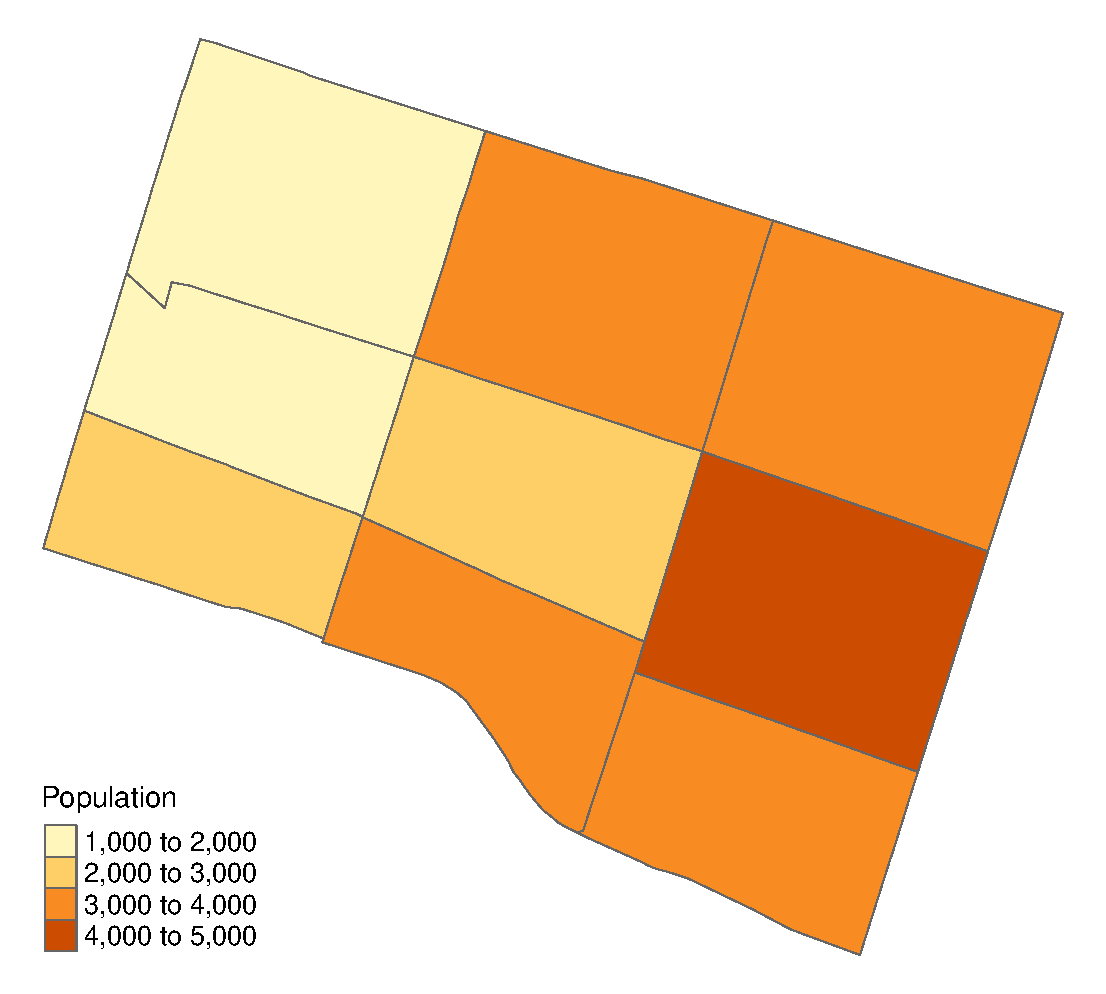
\includegraphics[width=1\linewidth]{Plots/map_population.pdf}  
  \caption{Population}
\end{subfigure}\hfill
\begin{subfigure}{0.48\textwidth}
  \centering
  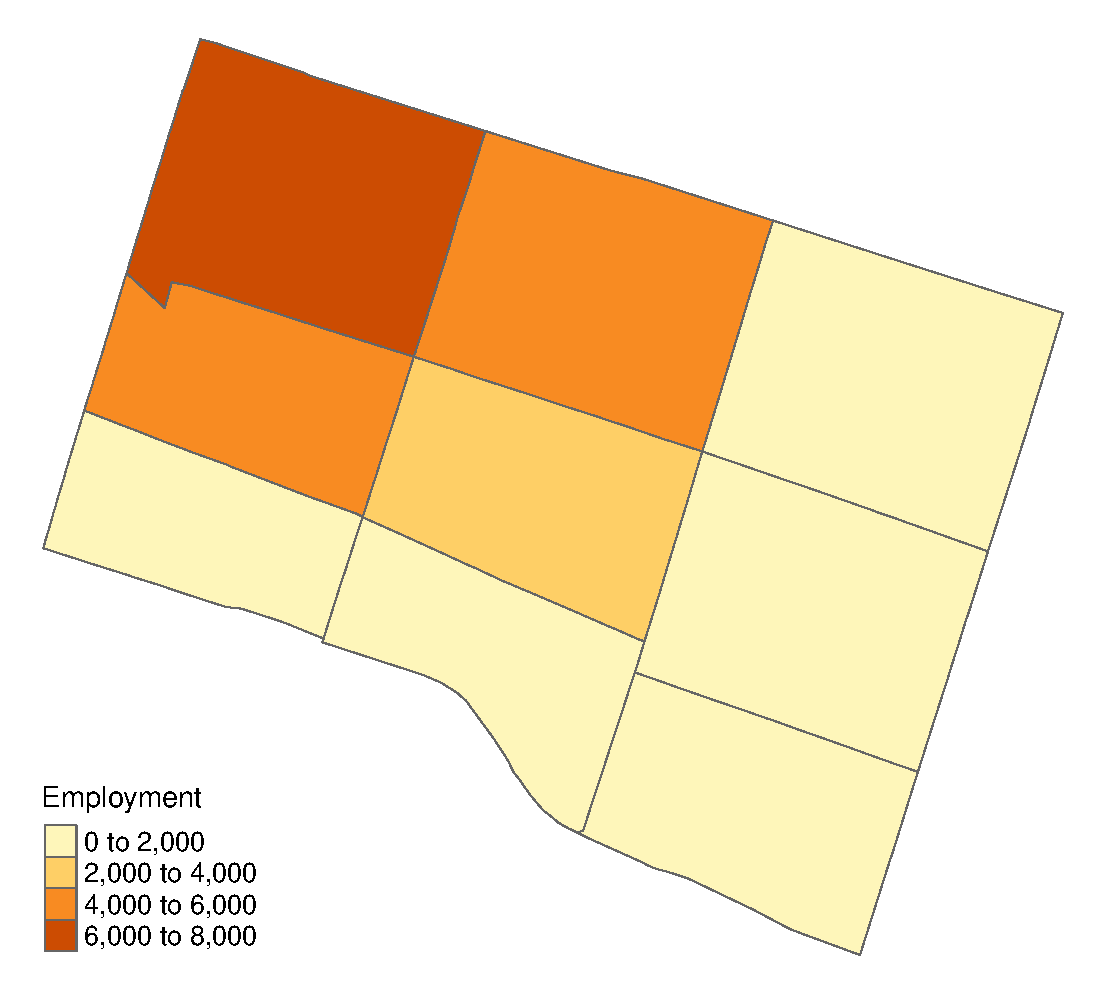
\includegraphics[width=1\linewidth]{Plots/map_employment.pdf}  
  \caption{Employment (jobs) }
\end{subfigure}\vspace{10pt}
 \begin{subfigure}{\textwidth}
  \centering
  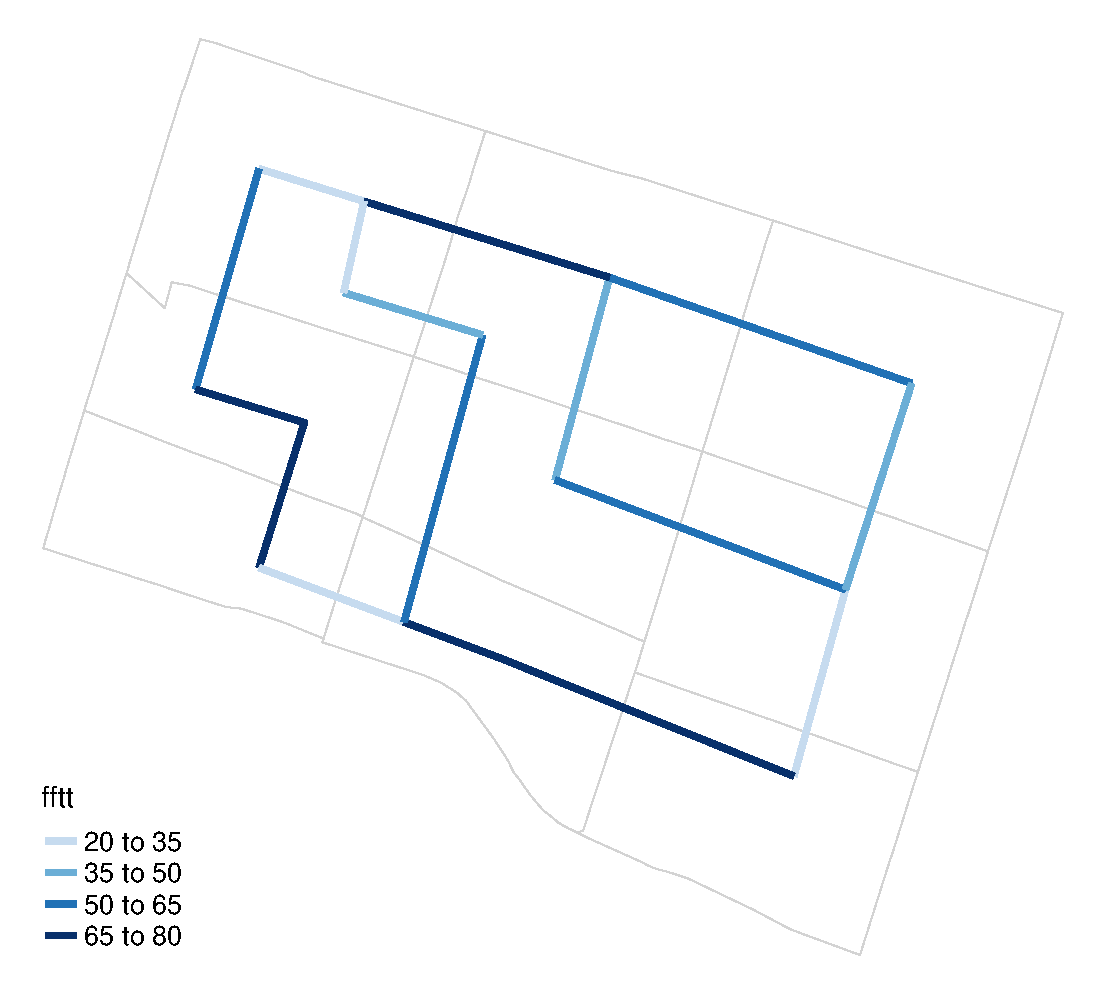
\includegraphics[width=0.48\linewidth]{Plots/map_network.pdf}  
  \caption{Free flow travel time (seconds)}
\end{subfigure}
\caption{Key information for reproducible example}
  \label{map-data-reproducible-example}
\end{figure}

Accessibility is calculated for this system based on Equation
(\ref{f:acc_empl}), using free flow travel time (\(fftt\)) on the
network as a measure of cost, and the following negative exponential
impedance function: \[
f(fftt_{ij}) = exp(-0.05\cdot fftt_{ij})
\]

Accessibility calculations results are shown in Fig.
\ref{accessibility-reproducible-example}, where it can be seen that
accessibility is high in more central locations and low in peripheral
locations, especially when network travel time to reach other zones is
long.

\begin{figure}
  \centering
  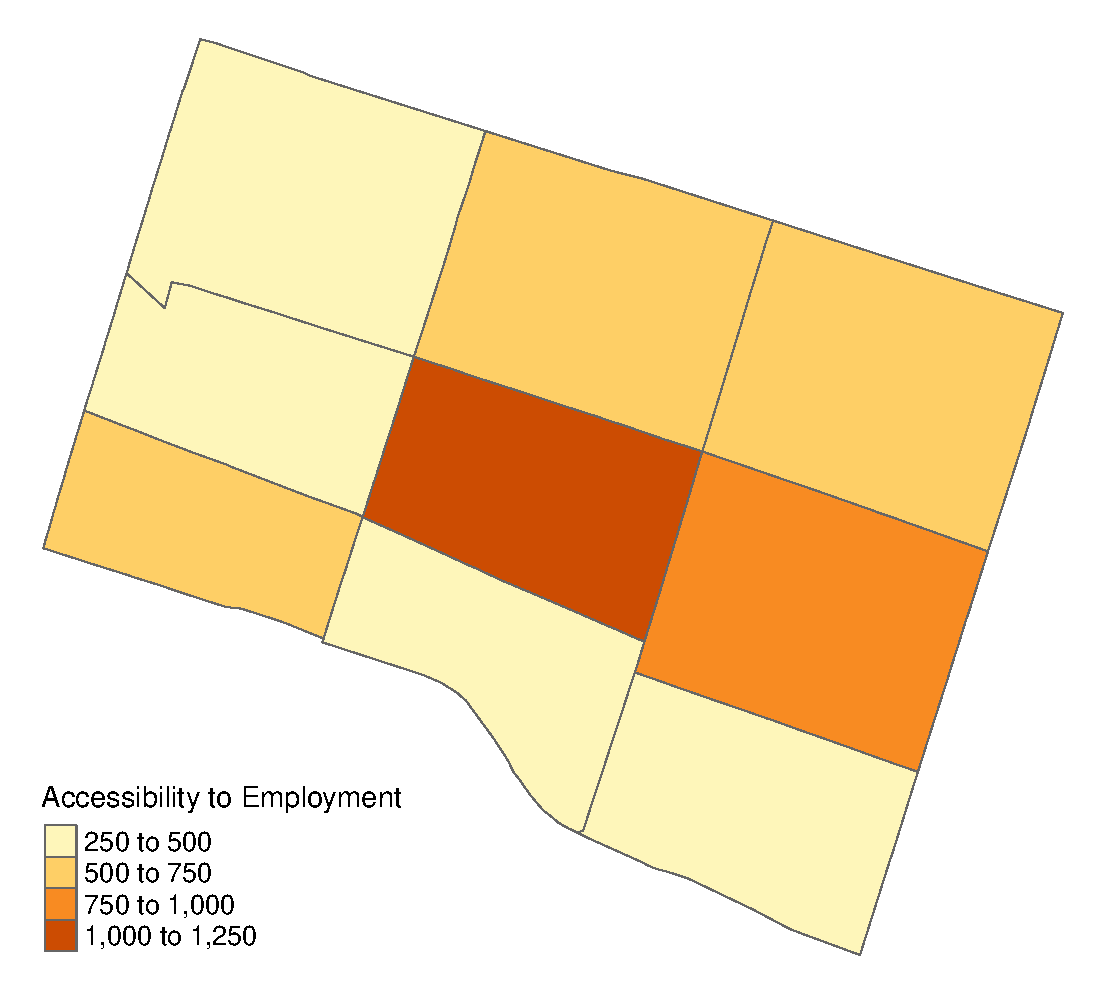
\includegraphics[width=0.8\linewidth]{Plots/map_accessibility.pdf}  
  \caption{Accessibility in reproducible example}
  \label{accessibility-reproducible-example}
\end{figure}

Calculation of betweenness-accessibility involves finding the shortest
paths from each origin to every potential destination. Shortest paths
are found using travel time in the network. Fig.
\ref{shortest-paths-example} shows the shortest path trees from each
node. Once the shortest paths have been identified, it is possible to
allocate the potential for interaction to the network, according to
levels of employment accessibility, as described in formula
(\ref{f:btw_pop}).

Consider, for example, Panel (a) in Fig. \ref{shortest-paths-example}.
This panel displays the shortest path tree from Node 1 (i.e., the
centroid of Zone 1) in the northwest corner of the system. This zone,
with a population of \(1,658\), ``pushes'' \(1,314.55\) people on the
link between Nodes 1 and 3. Of these, \(8.29\) continue on the link to
Node 4. Put another way, Zone 3 is ``pulling'' \(1,306.26\) workers from
Zone 1, and Zone 4 is pulling \(8.29\) workers from Zone 1. Similarly,
Zone 1 is pushing \(340.46\) people on the first segment of the network
in the Node 2 direction. Of these, \(336.13\) continue to Node 2 and
\(7.33\) to Node 8. Of those that continued to Node 8, only \(0.21\)
proceed to Node 5. Similarly, \(4.63\) of those who continued to Node 2
advance to Node 7 and \(31.66\) to Node 6. Finally, only \(0.86\) of
those that reached Node 6 advance to Node 11 - or alternatively, the
number of workers ``pulled'' by Node 11 (i.e., Zone 9) from Zone 1 is
only \(0.86\). As seen in this panel, network links between Nodes 7 and
11, between Nodes 5 and 11, and between 4 and 8, do not accommodate any
potential flow-through originating in Zone 1.

\begin{figure}
\begin{subfigure}{0.32\textwidth}
  \centering
  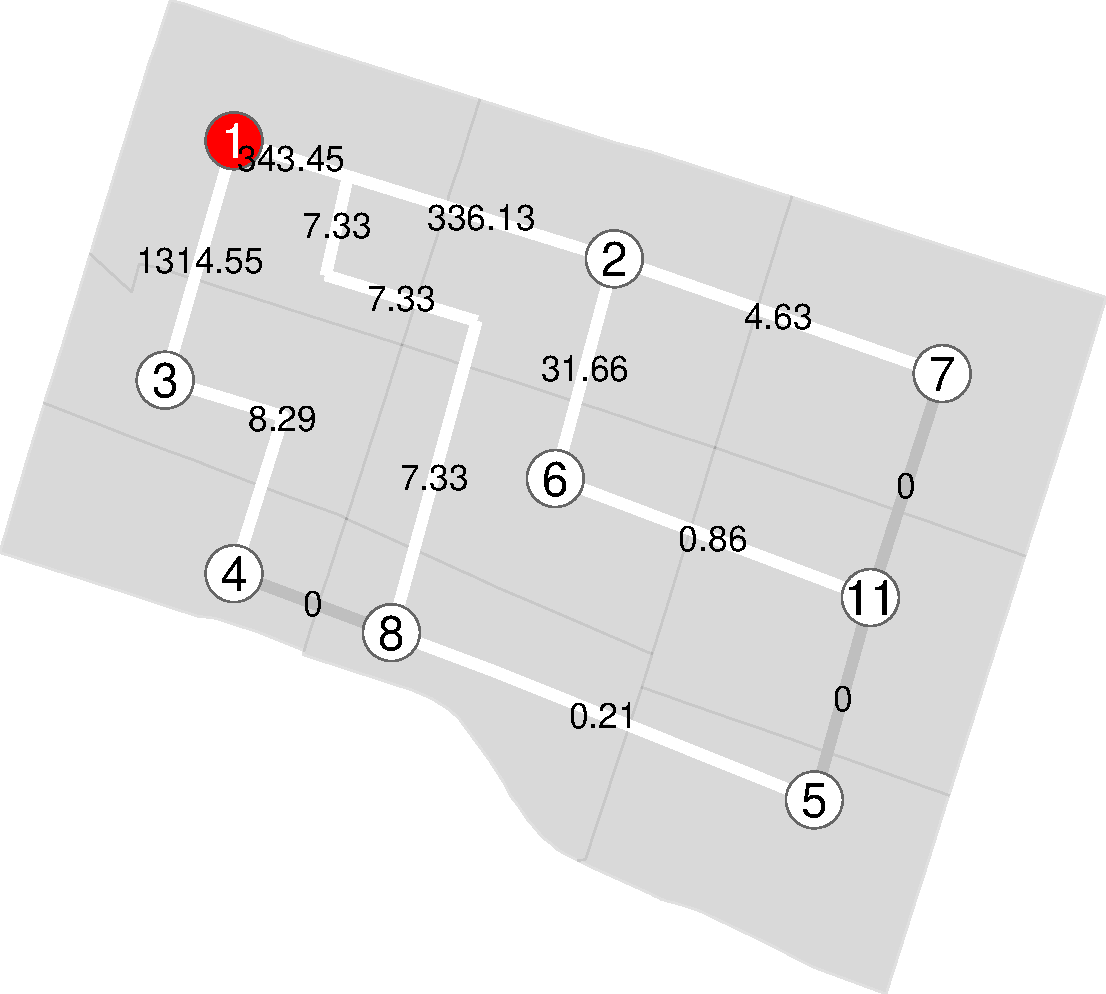
\includegraphics[width=1\linewidth]{Plots/sp1.pdf}  
  \caption{Node 1}
\end{subfigure}
\begin{subfigure}{0.32\textwidth}
  \centering
  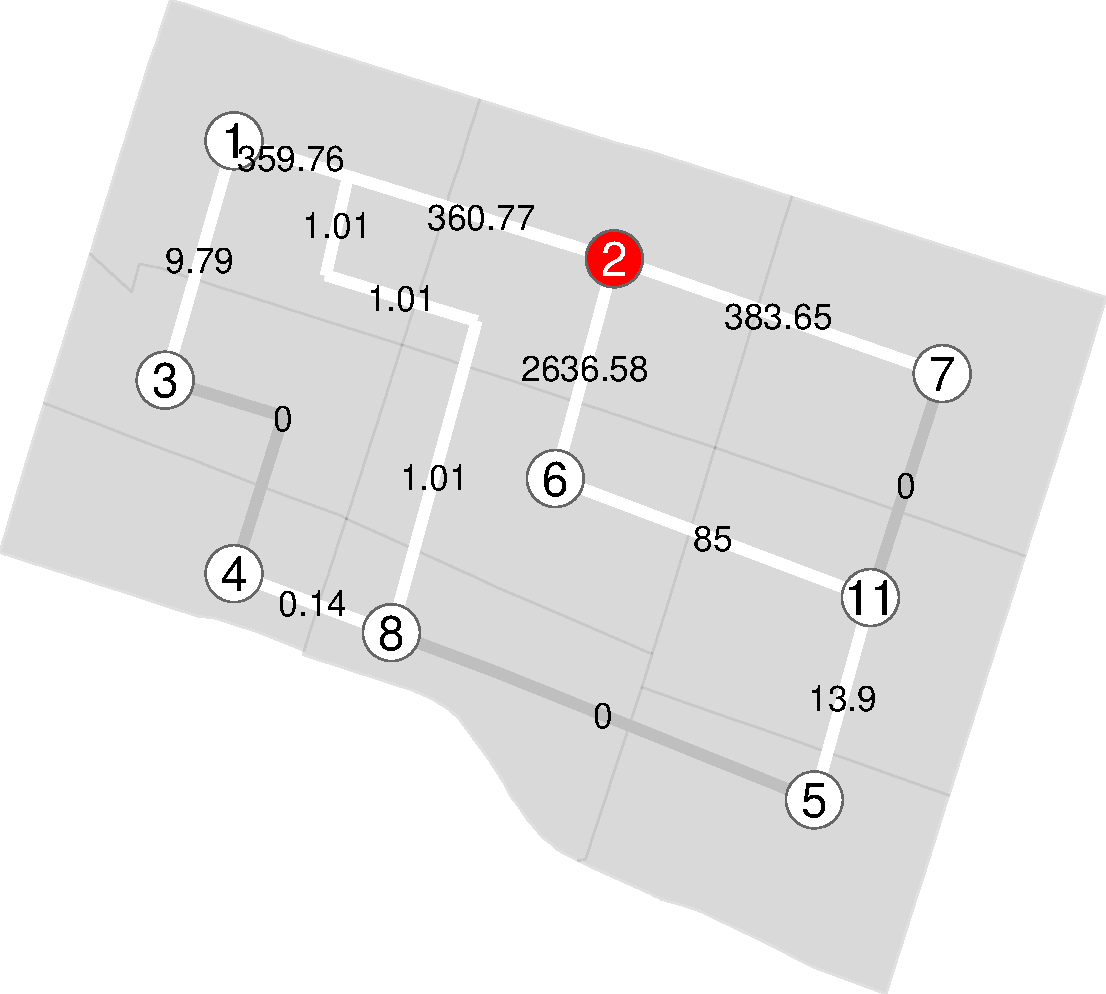
\includegraphics[width=1\linewidth]{Plots/sp2.pdf}  
  \caption{Node 2}
\end{subfigure}
 \begin{subfigure}{0.32\textwidth}
  \centering
  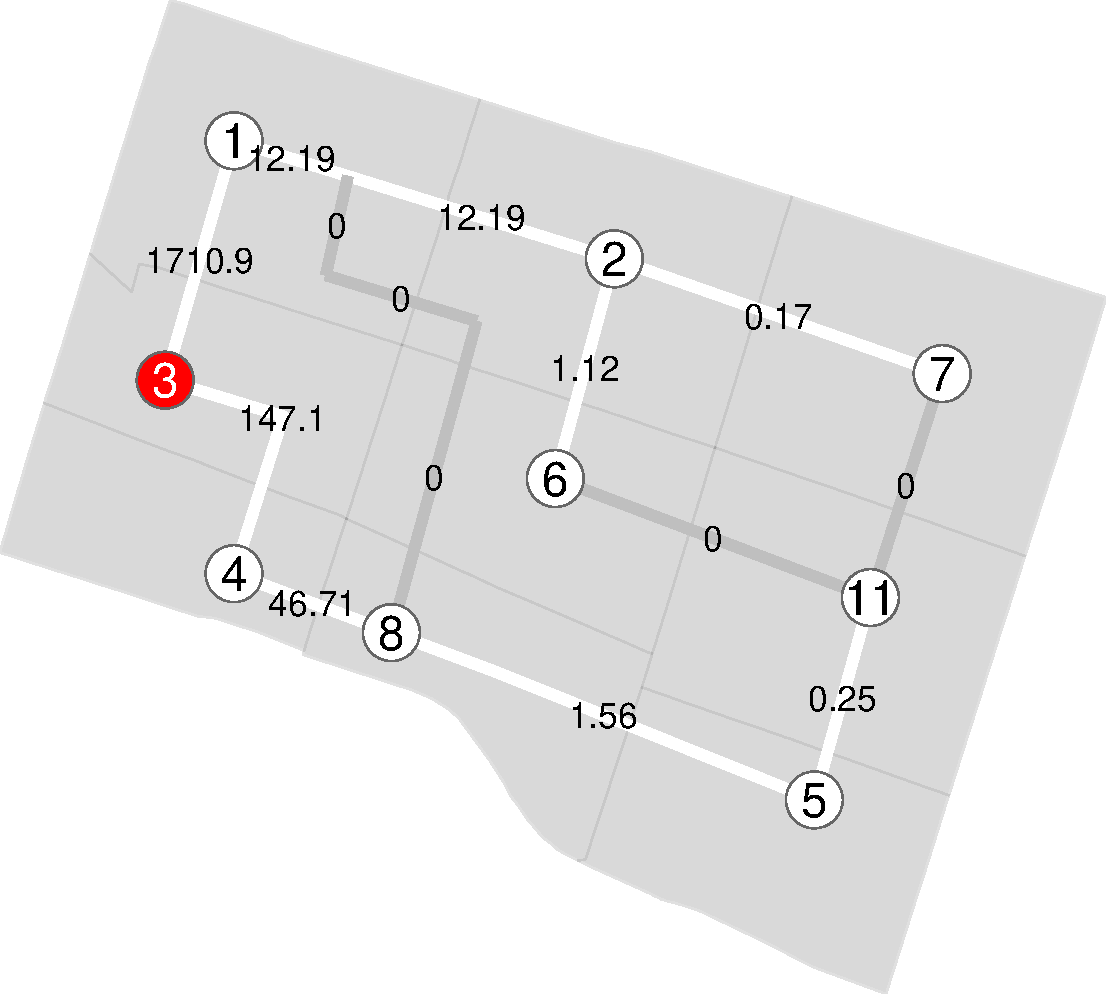
\includegraphics[width=1\linewidth]{Plots/sp3.pdf}  
  \caption{Node 3}
\end{subfigure}
\begin{subfigure}{0.32\textwidth}
  \centering
  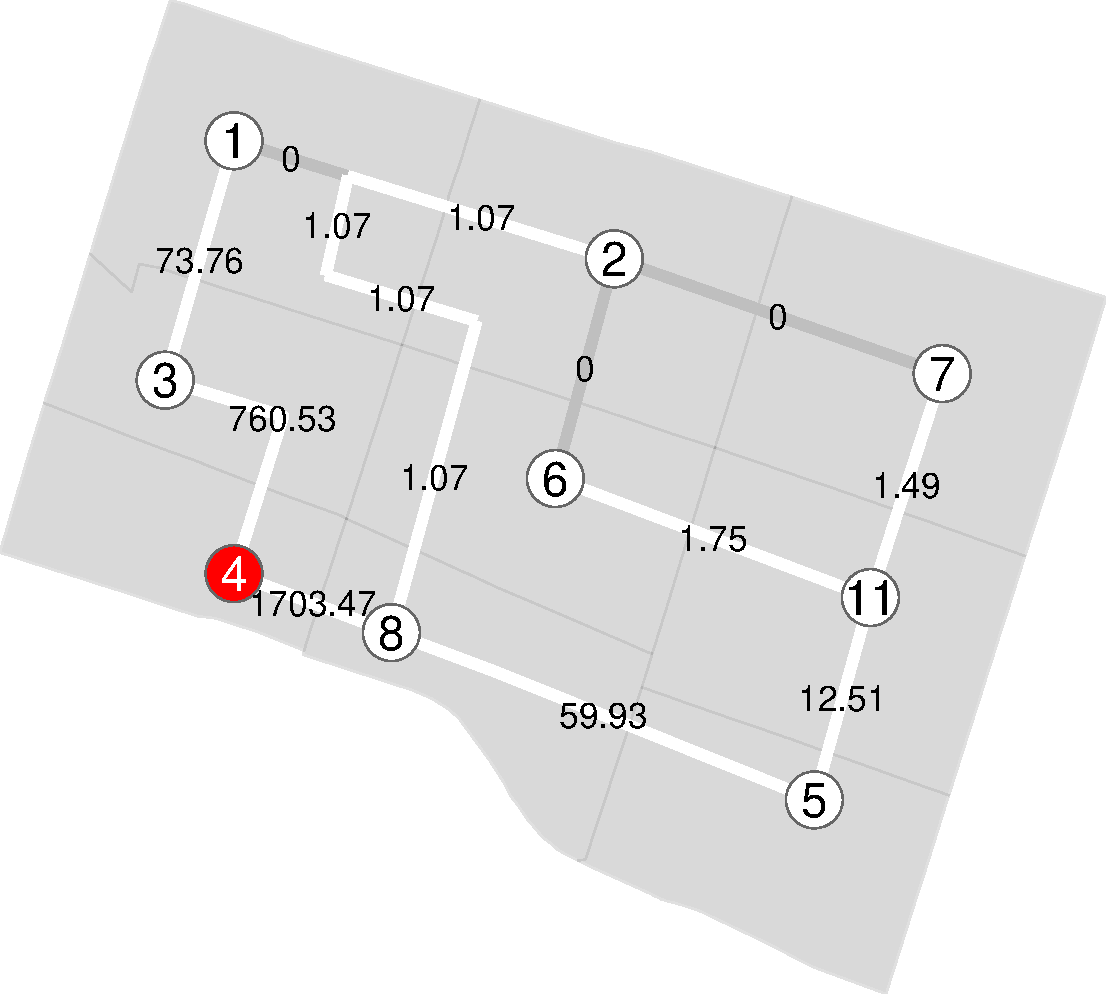
\includegraphics[width=1\linewidth]{Plots/sp4.pdf}  
  \caption{Node 4}
\end{subfigure}
\begin{subfigure}{0.32\textwidth}
  \centering
  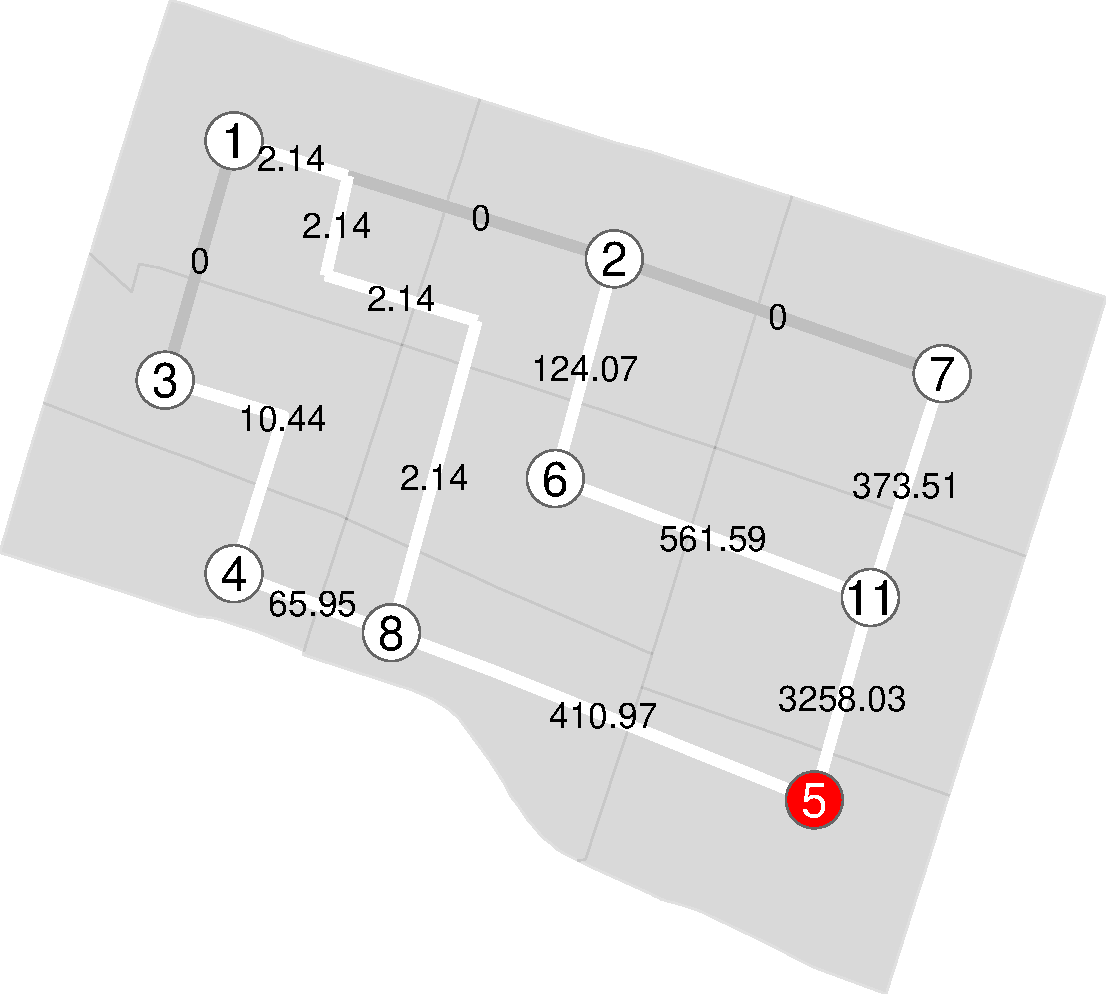
\includegraphics[width=1\linewidth]{Plots/sp5.pdf}  
  \caption{Node 5}
\end{subfigure}
\begin{subfigure}{0.32\textwidth}
  \centering
  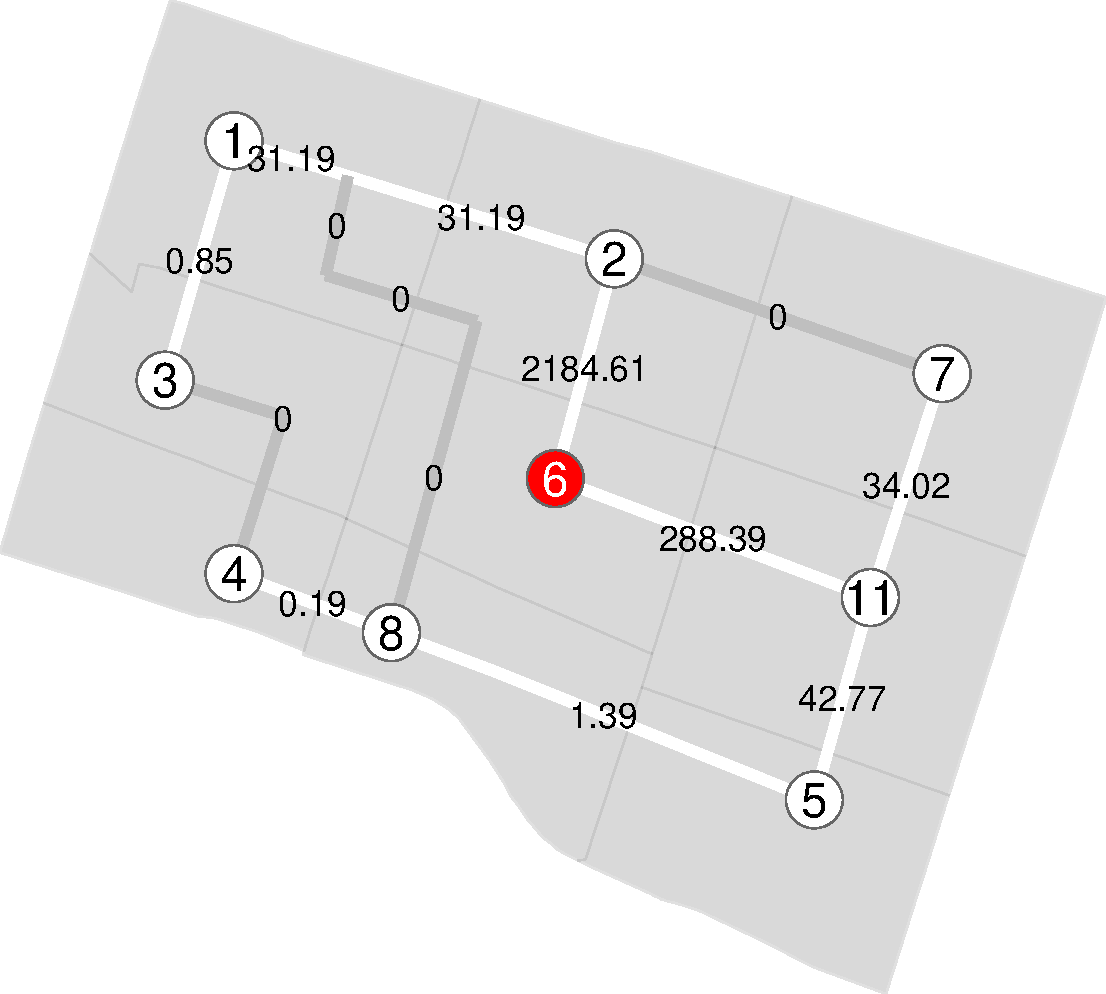
\includegraphics[width=1\linewidth]{Plots/sp6.pdf}  
  \caption{Node 6}
\end{subfigure}
\begin{subfigure}{0.32\textwidth}
  \centering
  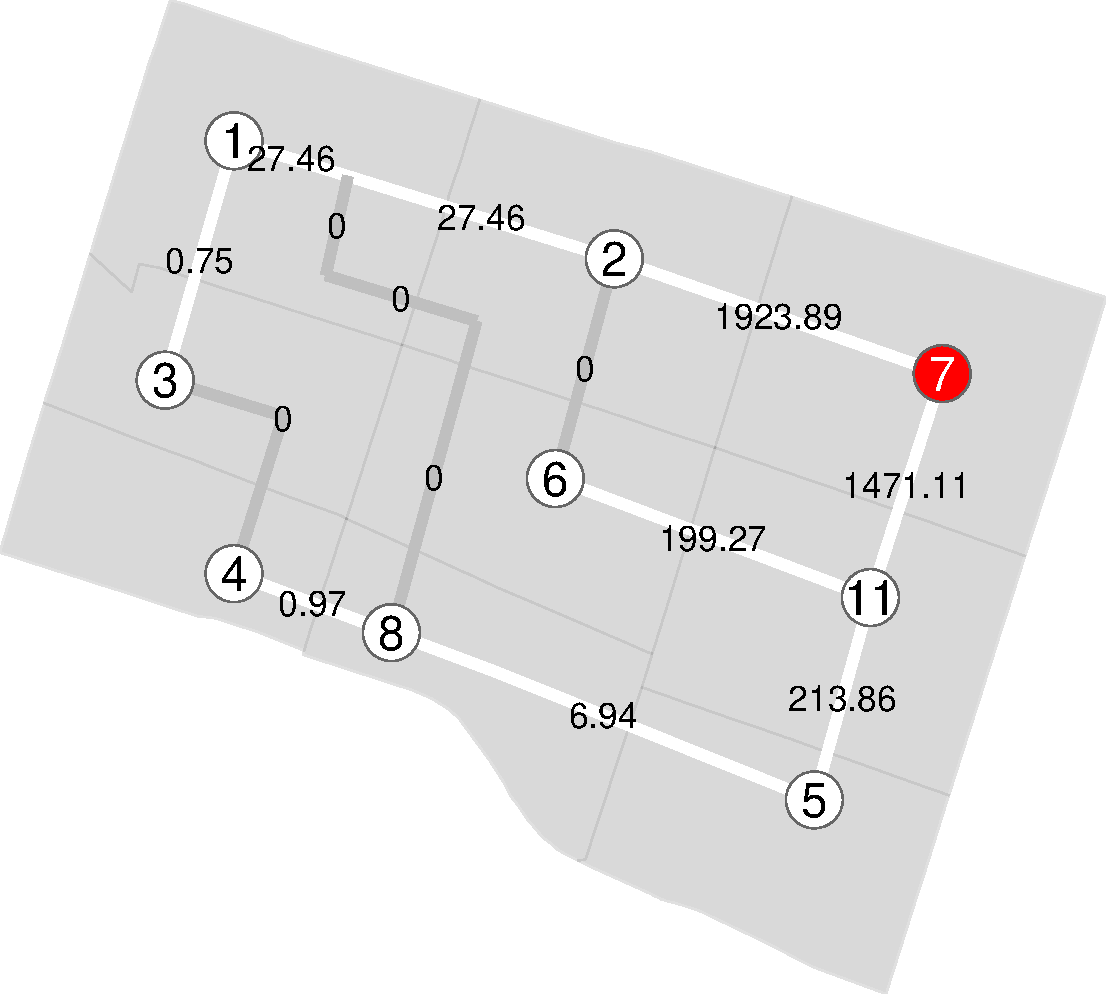
\includegraphics[width=1\linewidth]{Plots/sp7.pdf}  
  \caption{Node 7}
\end{subfigure}
\begin{subfigure}{0.32\textwidth}
  \centering
  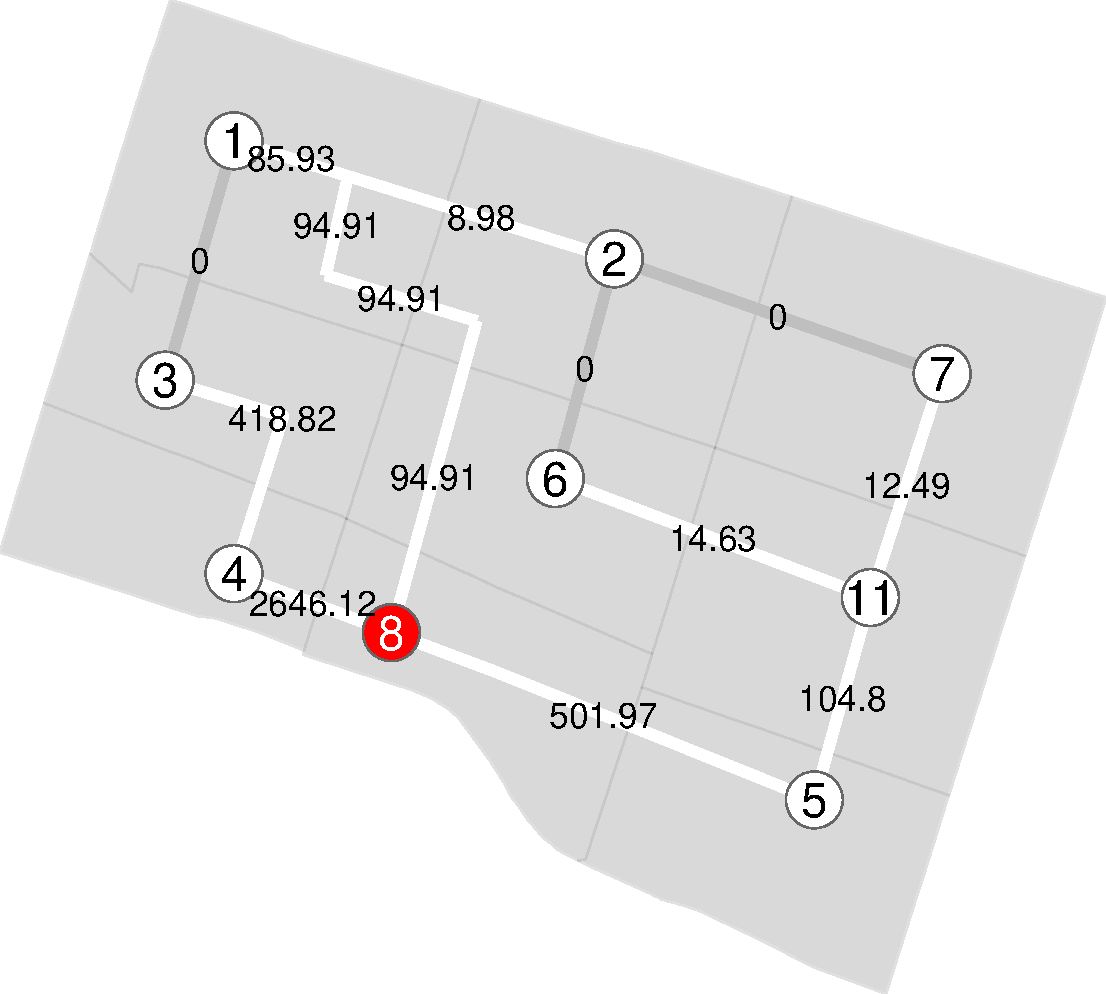
\includegraphics[width=1\linewidth]{Plots/sp8.pdf}  
  \caption{Node 8}
\end{subfigure}
\begin{subfigure}{0.32\textwidth}
  \centering
  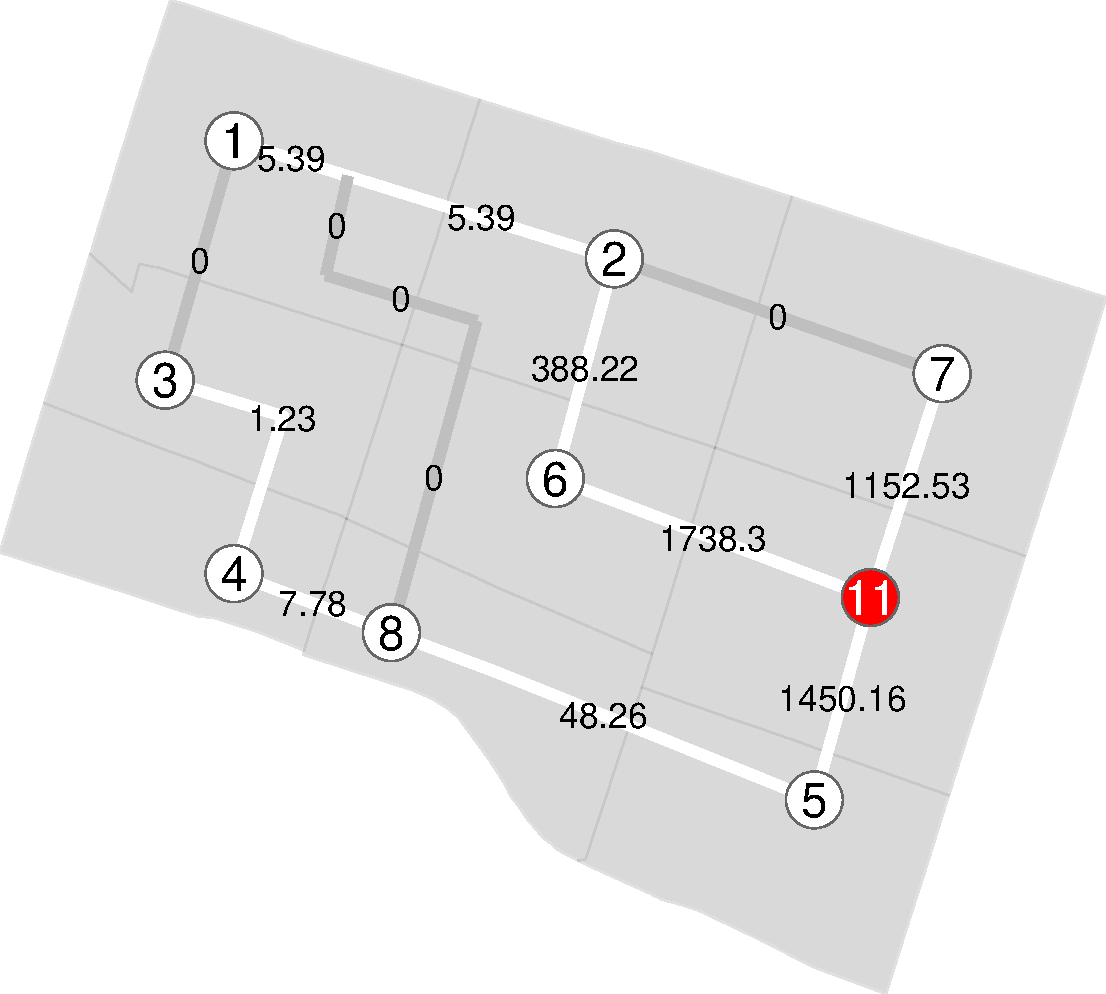
\includegraphics[width=1\linewidth]{Plots/sp11.pdf}  
  \caption{Node 11}
\end{subfigure}
\caption{Shortest paths and contributions to betweenness-accessibility by node}
  \label{shortest-paths-example}
\end{figure}

The rest of the panels in Fig. \ref{shortest-paths-example} provide a
similar breakdown of the way flow-throughs are allocated for each zone
of origin. Betweenness-accessibility is the total sum of all network
flows after this process is completed for every origin zone. Results are
shown in Fig. \ref{btw-accessibility-reproducible-example}, where
potential volume for each network link can be seen as an incidental
effect of accessibility.

\begin{figure}
  \centering
  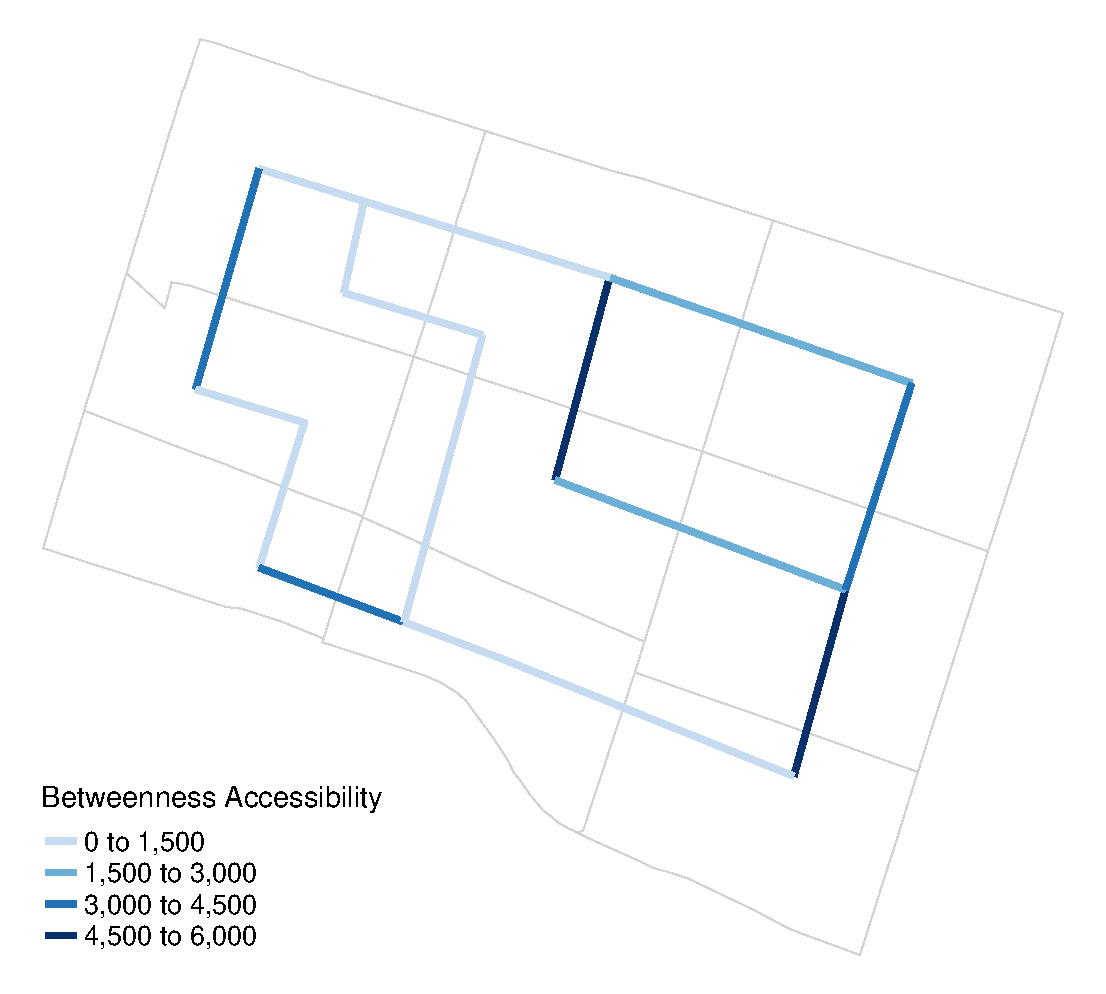
\includegraphics[width=0.8\linewidth]{Plots/map_btw.pdf}  
  \caption{Betweenness-accessibility in reproducible example}
  \label{btw-accessibility-reproducible-example}
\end{figure}

\hypertarget{case-study}{%
\section{Case study}\label{case-study}}

\hypertarget{context-and-data-sources}{%
\subsection{Context and data sources}\label{context-and-data-sources}}

In this section, we present an application of betweenness-accessibility
in a real-life urban network. This allows us to examine different
aspects of the proposed measures, along with their potential utility in
practice. The case study is the city of Zurich - the largest city in
Switzerland with a population of over 400,000 at the center of a
metropolitan area with a population of almost 1.4 million\footnote{Statistical
  Data on Switzerland 2018, Federal Statistical Office}. In addition to
its role as a major city in Switzerland, Zurich is one of the main
economic hubs in central Europe. We use a detailed network of
navigation-quality, commercially available from Tom-Tom. The network
includes all links and nodes within city boundaries. In addition, to
minimize the impact of boundary effects, the case study includes a
buffer area of two kilometers. The resulting network consists of over
\(48,000\) links and \(23,000\) nodes (see Fig. \ref{network}).

\begin{figure}
  \centering
  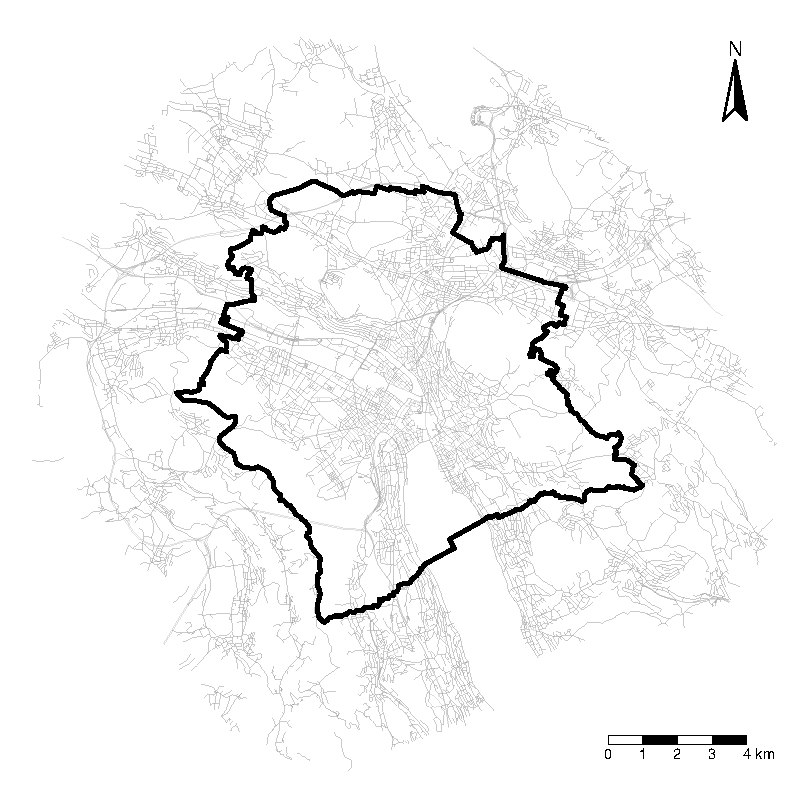
\includegraphics[width=0.6\linewidth]{Plots/network_overview.pdf}  
  \caption{Network overview and city boundaries}
  \label{network}
\end{figure}

As discussed, betweenness-accessibility provides a bridge between the
concepts of betweenness (from social network analysis) and accessibility
(from transport geography). Therefore, in addition to network data, we
also need population and employment data for the relevant accessibility
calculations. It is important to note that more disaggregated data
increases the computational cost of the indicator, since the number of
shortest paths grows quadratically with the number of
origins/destinations (i.e., \(N(N-1)\) shortest paths for a directed
network with \(N\) nodes). For the case study, we use the zoning system
of the Swiss National Transport Model\footnote{NPVM 2015, ARE}. The city
of Zurich is divided into 308 zones with sizes ranging from 0.02 to 3.89
\(km^2\) (mean value of 0.30 \(km^2\)). The population and employment
data are for the year 2015; identification and processing of
\(308\times307=94'556\) shortest paths is required for construction of
introduced indicators. To account for spatial opportunities distribution
within each zone, we randomly assign a node within each zone as the
starting and ending node. All shortest path calculations use free-flow
travel time; these are used to construct the origin-destination (O-D)
travel time matrix, a prerequisite for accessibility calculations.

The distance decay function is calibrated using the survival analysis
method presented in Sarlas and Axhausen (2018). For this, we employ data
from a household survey\footnote{Swiss Micro-census 2015, ARE}, using
observations of individuals living and working in Zurich and commuting
by car. Individuals' home and work locations are matched to the
corresponding zones. Subsequently, we utilize the previously constructed
O-D travel time matrix to obtain the survival function of trip length
within the boundaries of the city. In the next step, we fit a negative
exponential function to the trip length function to give the following
calibrated distance decay function:

\[
f(tt_{ij})=exp({{\beta} \cdot tt_{ij}^{\alpha}})
\]

with \({\alpha}=3.5875\), \({\beta}=-6.164*10^{-4}\), and \(tt\) the
free flow travel time in minutes.

After completing the analysis of accessibility and identification of the
required shortest paths, the next step is to calculate the normalized
betweenness-accessibility indicators (Equations
\ref{f:btw_pop},\ref{f:btw_empl},\ref{f:btw_acc_pop},and
\ref{f:btw_empl_pop}). For comparison purposes, we also calculate and
present results of the conventional betweenness indicator
\(C_{\rm B}^{\rm N}\). Apart from that, the \(C_{\rm B_{OD}}^{\rm N}\)
indicator is also calculated. Recall that \(C_{\rm B_{OD}}^{\rm N}\) is
the equivalent to \(C_{\rm B}^{\rm N}\) but only for a subset of
interacting nodes; in this particular case we use the \(308\times 307\)
shortest paths, and normalize them by means of the total number of
shortest paths (i.e., \(308\times 307=94'556\)).

All analysis described was performed using \texttt{R} (R 2013), and
utilizing the \textit{igraph} package (Csardi and Nepusz 2006),
customized with additional functions to calculate the various
indicators. This analysis is conducted for links, but similar analysis
can be conducted for nodes with only minor adjustments to the
calculations.

\hypertarget{calculation-of-indicators}{%
\subsection{Calculation of indicators}\label{calculation-of-indicators}}

The indicators are shown in Figures \ref{plots_ntw} and
\ref{centralities}). It is interesting to see that the different
indicators show disparate pictures of the importance of links. A
comparison between \(C_{\rm B}^{\rm N}\) and \(C_{\rm B_{OD}}^{\rm N}\)
(Fig. \ref{plots_ntw}) for the whole network shows that, in the former,
links on the periphery - along with some in the central area of Zurich -
are relatively more important. For \(C_{\rm B_{OD}}^{\rm N}\), however,
important links are fully concentrated in the central parts of the city.
The range of values is also interesting, since it indicates that \(1\%\)
of links with the highest values per case have relative shares of
\(4.19-9.21\%\) and \(3.42-9.21\%\) of the total shortest paths passing
through them.

To better appreciate the differences between \(C_{\rm B_{OD}}^{\rm N}\)
and betweenness-accessibi-lity indicators we focus on the central area
of Zurich (Fig. \ref{centralities}). At first, all indicators appear to
yield similar results. However, differences can be identified especially
with respect to the corresponding shares. For \(C_{\rm pop}^{\rm N}\),
the highest \(1\%\) of links have a a potential number of users in a
range of \(3.22-7.5\%\) of the total city population. For
\(C_{\rm empl}^{\rm N}\), the corresponding relative share is
\(3.01-8.21\%\), revealing a higher share of total employment positions.
The results of indicators \(C_{A_{\rm pop}}^{\rm N}\) and
\(C_{A_{\rm empl}}^{\rm N}\) are similar, but slightly lower.
Interestingly, it appears that connectivity generated through specific
links produces almost \(6.8\%\) and \(6.4\%\), respectively, of total
accessibility per case.

\begin{figure}
\centering
\begin{subfigure}{.45\textwidth}
  \centering
  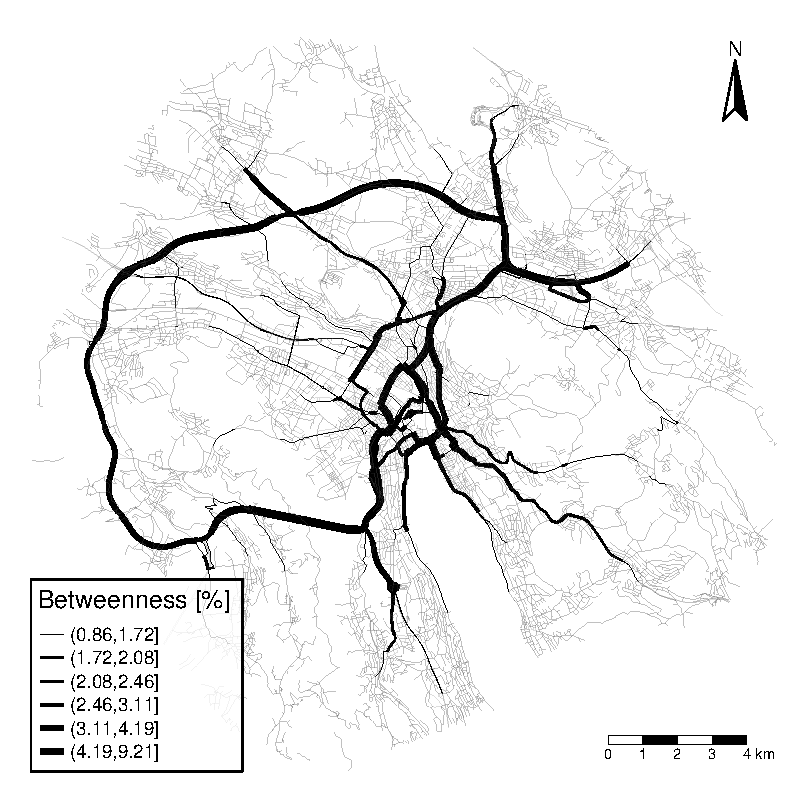
\includegraphics[width=1\linewidth]{Plots/btw.pdf}  
  \caption{$C_{\rm B}^{\rm N}$}
\end{subfigure}
\begin{subfigure}{.45\textwidth}
  \centering
  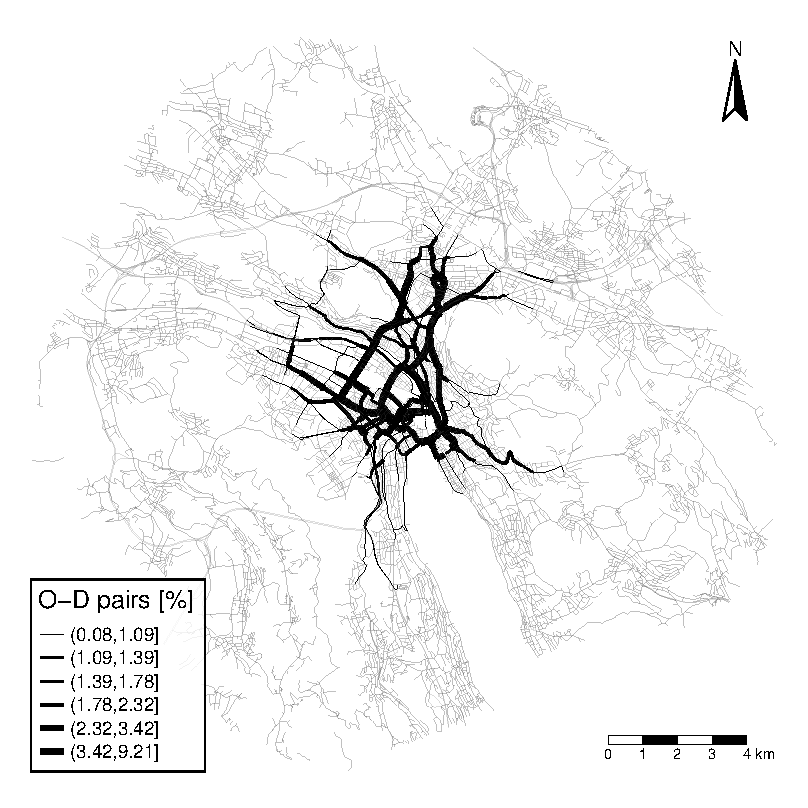
\includegraphics[width=1\linewidth]{Plots/od.pdf}  
  \caption{$C_{\rm B_{OD}}^{\rm N}$}
\end{subfigure}
 \caption{Comparison of $C_{\rm B}^{\rm N}$ and $C_{\rm B_{OD}}^{\rm N}$ indicators' results}
  \label{plots_ntw}
\end{figure}

\begin{figure}
\begin{subfigure}{.5\textwidth}
  \centering
  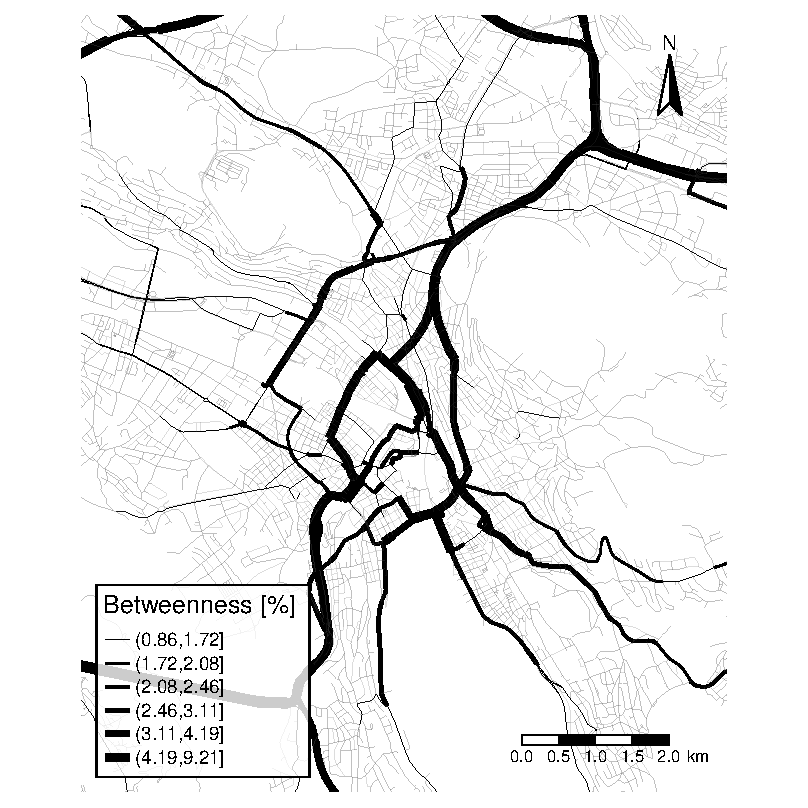
\includegraphics[width=1\linewidth]{Plots/btw_center.pdf}  
  \caption{$C_{\rm B}^{\rm N}$}
\end{subfigure}
\begin{subfigure}{.5\textwidth}
  \centering
  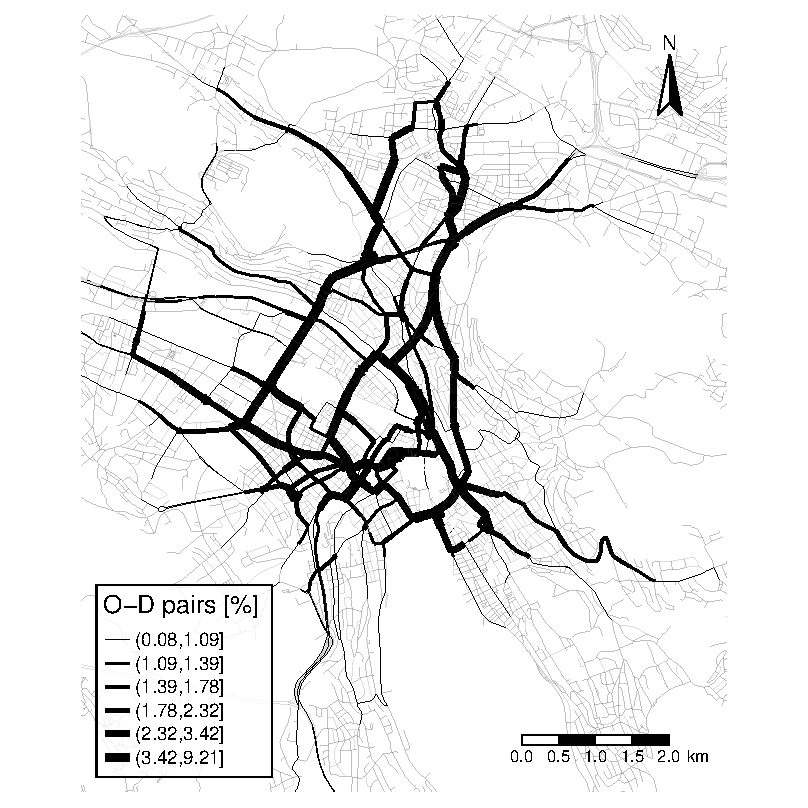
\includegraphics[width=1\linewidth]{Plots/od_center.pdf}  
  \caption{$C_{\rm B_{OD}}^{\rm N}$}
\end{subfigure}
 \begin{subfigure}{.5\textwidth}
  \centering
  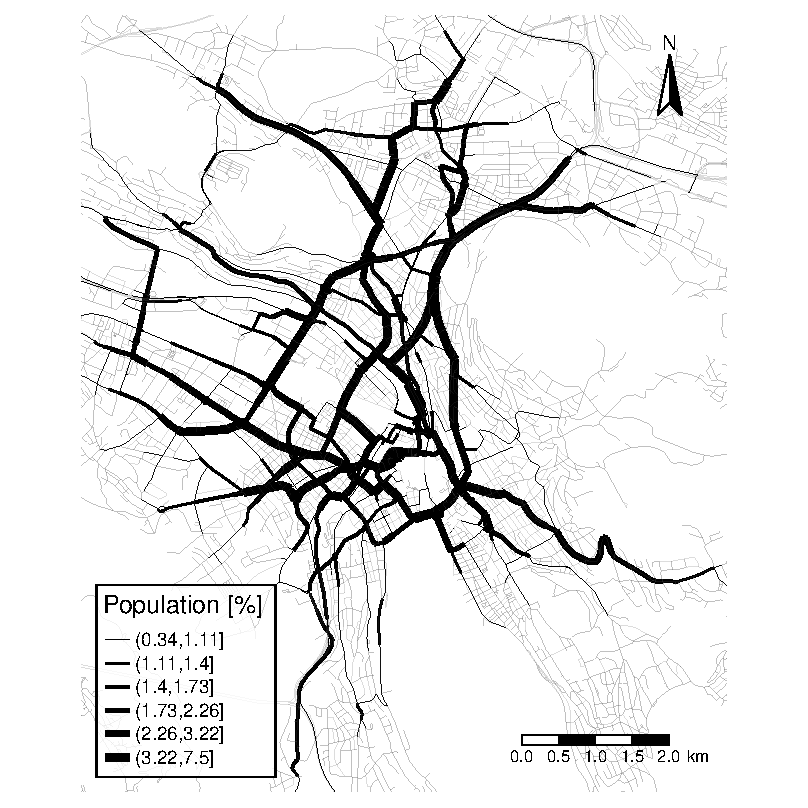
\includegraphics[width=1\linewidth]{Plots/empl_acc_pop_center.pdf}  
  \caption{$C_{\rm pop}^{\rm N}$}
\end{subfigure}
\begin{subfigure}{.5\textwidth}
  \centering
  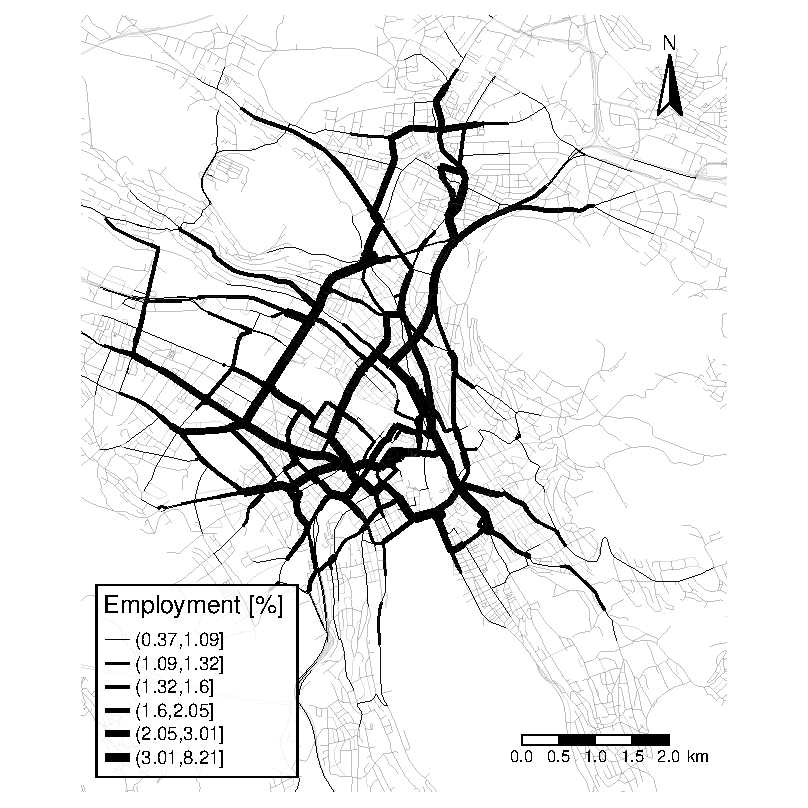
\includegraphics[width=1\linewidth]{Plots/pop_acc_empl_center.pdf}  
  \caption{$C_{\rm empl}^{\rm N}$}
\end{subfigure}
\begin{subfigure}{.5\textwidth}
  \centering
  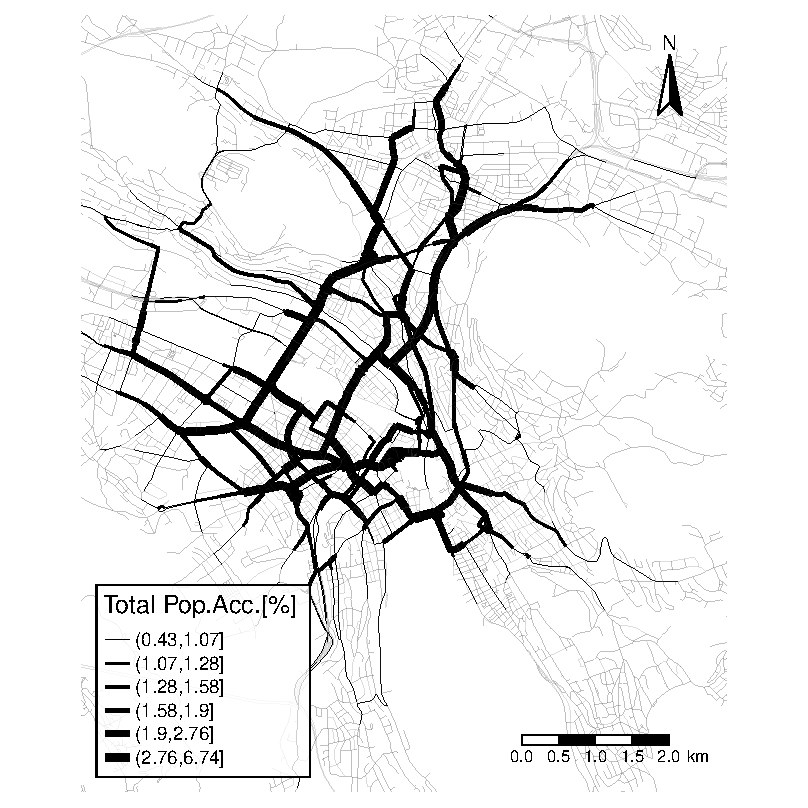
\includegraphics[width=1\linewidth]{Plots/pop_acc_center.pdf}  
  \caption{$C_{A_{\rm pop}}^{\rm N}$}
\end{subfigure}
\begin{subfigure}{.5\textwidth}
  \centering
  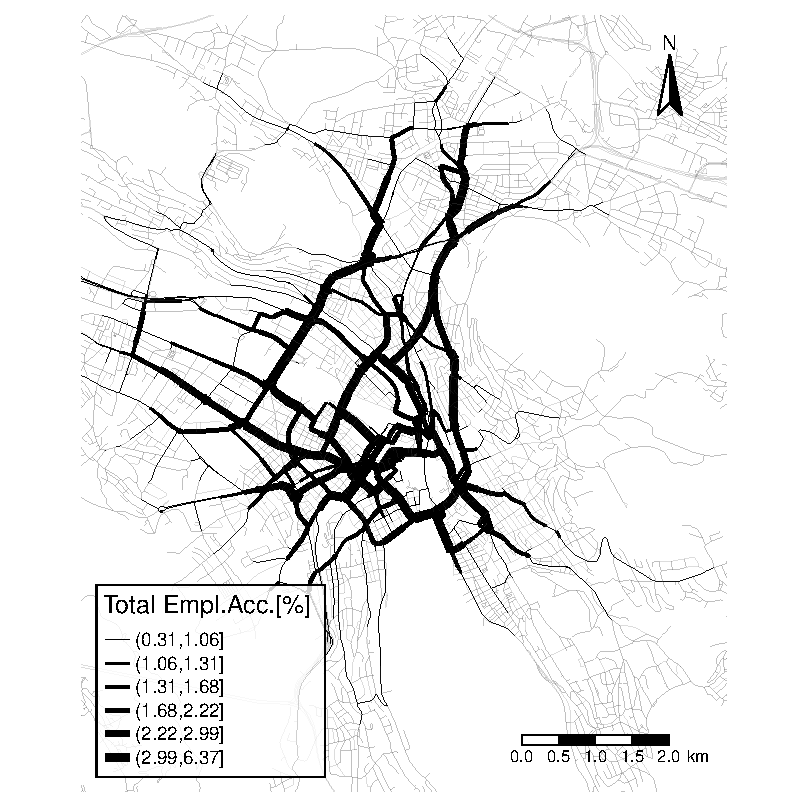
\includegraphics[width=1\linewidth]{Plots/empl_acc_center.pdf}  
  \caption{$C_{A_{\rm empl}}^{\rm N}$}
\end{subfigure}
\caption{Various centrality indicators' results}
  \label{centralities}
\end{figure}

Last, correlation analysis is used to explore how various indicators
relate to each other (see Table \ref{btw-correlation}). As seen in the
table, the conventional betweenness indicator has the lowest degree of
correlation with other indicators. This is not surprising, given the
substantial differences in their formulations - betweenness only
considers network topology, while other measures also consider flows on
the links (also see López et al. 2017). Other indicators tend to exhibit
higher correlations, despite using different weighting schemes. This can
perhaps be attributed to the fact that they all utilize the same sets of
shortest paths.

\begin{table}[!htbp] \centering 
    \small
    \caption{Correlation matrix of betweenness accessibility measures} 
    \label{btw-correlation} 
    \begin{tabular}{@{\extracolsep{1pt}} lrrrrrr} 
        \hline \\[-1.8ex] 
        & \multicolumn{1}{r}{$C^{\rm N}_{\rm B}$} & \multicolumn{1}{r}{$C^{\rm N}_{\rm B_{OD}}$} & \multicolumn{1}{r}{$C^{\rm N}_{\rm pop}$} & \multicolumn{1}{r}{$C^{\rm N}_{\rm empl}$} & \multicolumn{1}{r}{$C^{\rm N}_{\rm A_{empl}}$} & \multicolumn{1}{r}{$C^{\rm N}_{\rm A_{pop}}$} \\ 
        \hline \\[-1.8ex] 
        $C^{\rm N}_{\rm B}$ & $1$ & $0.63$ & $0.55$ & $0.55$& $0.54$ & $0.57$ \\ 
        $C^{\rm N}_{\rm B_{OD}}$ & $0.63$ &$1$ & $0.89$ & $0.91$ & $0.92$ & $0.96$ \\
        $C^{\rm N}_{\rm pop}$ & $0.55$ & $0.89$ &$1$ & $0.69$ & $0.93$ & $0.78$ \\
        $C^{\rm N}_{\rm empl}$ & $0.55$ & $0.91$ & $0.69$ & $1$& $0.83$ & $0.97$  \\ 
        $C^{\rm N}_{\rm A_{empl}}$ & $0.54$ & $0.92$ & $0.93$ & $0.83$ & $1$ & $0.86$  \\ 
        $C^{\rm N}_{\rm A_{pop}}$ & $0.57$ & $0.96$ & $0.78$ & $0.97$ & $0.86$ & $1$ \\ 
        \hline \\[-1.8ex] 
    \end{tabular} 
\end{table}

\hypertarget{application-of-betweenness-accessibility-to-vulnerability-analysis}{%
\section{Application of betweenness-accessibility to vulnerability
analysis}\label{application-of-betweenness-accessibility-to-vulnerability-analysis}}

As noted in the introduction, the use of accessibility as a tool to
understand robustness/vulnerability is an emerging topic of research
(Liao and Wee 2017). In this section, we turn our attention to the
application of betweenness-accessibility to assess the vulnerability of
links in a network - that is, the degree to which performance of the
network degrades when links are subjected to stress, or interdicted.
Previous research has measured the performance of networks using network
connectivity and travel time (e.g., Jenelius, Petersen, and Mattsson
2006; Scott et al. 2006). As well, different strategies have been
proposed to approach both network performance and interdiction,
including Holme et al. (2002), who use four different attack strategies
based on topological indicators. The use of betweenness-accessibility
sees the role of the network in terms of allowing users to reach
destinations, and therefore allows us to study the socio-economic
impacts of a network's degradation (see Taylor, Sekhar, and D'Este 2006,
@Chen2007; Sohn 2006; Taylor 2017).

To test the ability of betweenness-accessibility to evaluate
vulnerability, we study the performance of the network subject to
attacks on its links (edges). As highlighted by Holme et al. (2002),
this approach (so-called ``attack vulnerability'') quantifies how
network performance declines when specific elements of the network are
removed (Barabási and Réka 1999). For the present case, the attack
strategy uses the ranking of the links in terms of six indicators (i.e.,
two betweenness centrality and four betweenness-accessibility
indicators). In addition, each attack happens in increments of five
links; in total, we run fifteen steps (i.e., attacks) in this
experiment. In pseudo-code, the experiment is presented in Algorithm
\ref{pseudo}.

\begin{algorithm}
\caption{Attack vulnerability experiment}
\begin{algorithmic}[1]
\For {$i=1$ to $6$ indicators}
\State Initialize full network
\State Calculate indicator $i$ 
\For {$j=1$ to $15$ attacks}
\State Remove current network's five most important links b.o. indicator $i$
\State Calculate performance $P_i^j$ of current network
\EndFor
\EndFor
\end{algorithmic}
\label{pseudo}
\end{algorithm}

As seen there, the performance of the network is assessed after each
attack. To that end, two approaches are used for the evaluation. The
first approach is accessibility-based; accordingly, we measure changes
in system-wide accessibility. The second approach measures changes in
system-wide travel time; optimal travel times are calculated using the
well-known transportation problem (Horner 2002; Scott, Kanaroglou, and
Anderson 1997). To implement the transportation problem, the number of
residents per zone is scaled up proportionally to match the total number
of employment positions in Zurich. Subsequently, an optimization process
that minimizes total travel time system-wide is used to calculate the
corresponding demand matrix. To account for demand dimensionality, the
optimization problem is formulated as two distinct problems. In the
first one (denoted as population-employment scenario), zonal population
serves as trip production proxy and employment positions as trip
attraction one, and vice versa (denoted as employment-population
scenario). The results of various evaluation criteria for the six
measures are presented in Figures \ref{acc-diff5} and \ref{tt-diff5}.

\begin{figure}[h!]
\centering
    \begin{subfigure}{.7\textwidth}
        \centering
        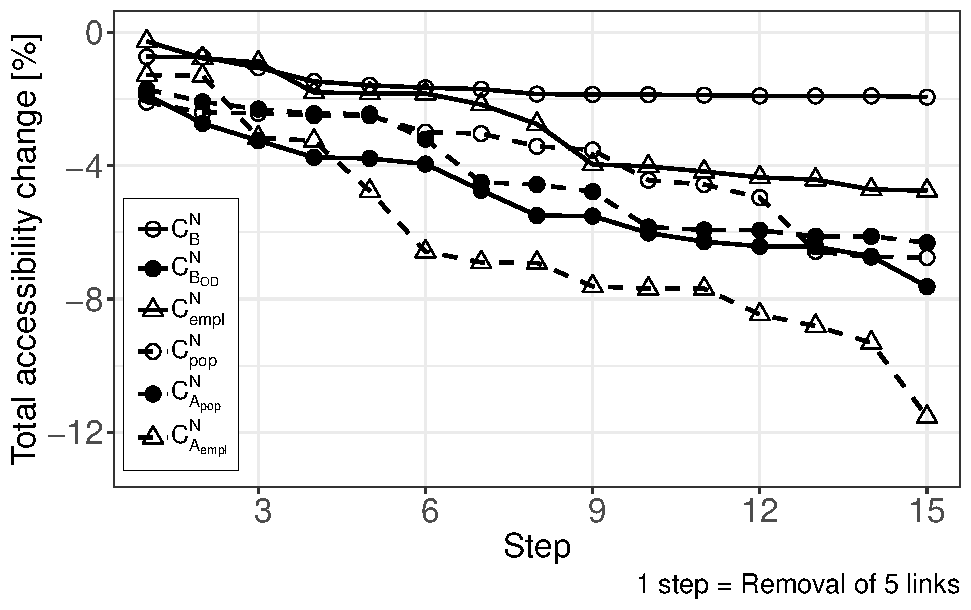
\includegraphics[width=1\linewidth]{Plots/acc_emp_5.pdf}  
        \caption{Employment accessibility}
        \label{acc-diff5a}
    \end{subfigure}
    \begin{subfigure}{.7\textwidth}
        \centering
        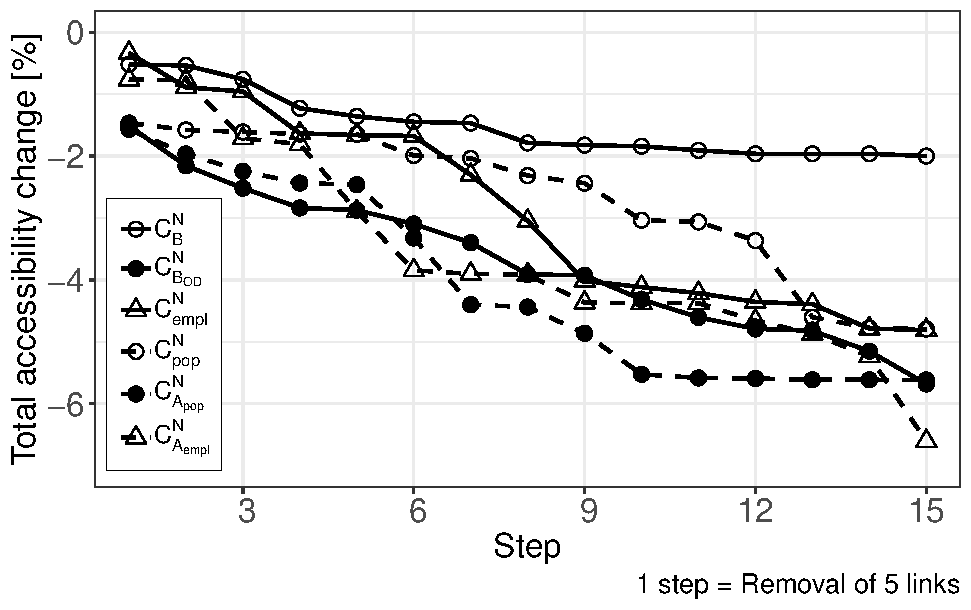
\includegraphics[width=1\linewidth]{Plots/acc_pop_5.pdf}  
        \caption{Population accessibility}
        \label{acc-diff5b}
    \end{subfigure}
    \caption{Accessibility-based performance indicator}
    \label{acc-diff5}
\end{figure}

\begin{figure}[!ht]
\centering
    \begin{subfigure}{.7\textwidth}
        \centering
        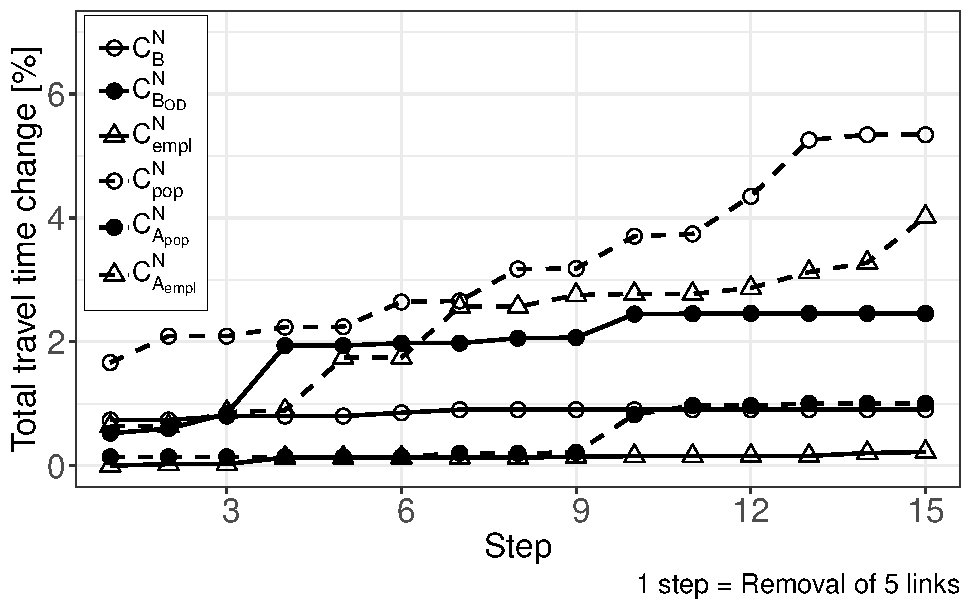
\includegraphics[width=1\linewidth]{Plots/travel_time_diff_5.pdf}  
        \caption{Population-employment scenario}
        \label{tt-diff5a}
    \end{subfigure}
    \begin{subfigure}{.7\textwidth}
        \centering
        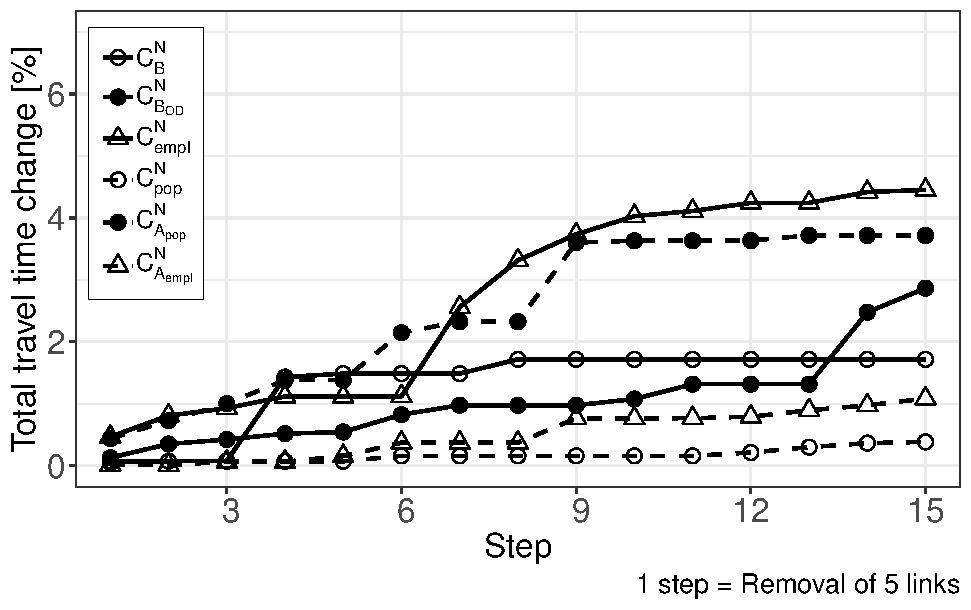
\includegraphics[width=1\linewidth]{Plots/travel_time_diff_5_emp.pdf}  
        \caption{Employment-population scenario}
        \label{tt-diff5b}
    \end{subfigure}
    \caption{Total travel-time performance indicator}
    \label{tt-diff5}
\end{figure}

As seen in Figure \ref{acc-diff5}, the network deteriorates much faster
- and to a greater extent - when attacks target links with high values
of betweenness-accessibility. Removing links based on the formulation
with embedded employment accessibility weights
(\(C_{A_{\rm empl}}^{\rm N}\)) has the highest impact on total
accessibility reduction. Particularly, for the employment accessibility
case (Fig. \ref{acc-diff5a}), reduction in accessibility levels is
substantial, almost \(12\%\), with a difference of about \(4\%\) from
the second best performing criterion. In addition, we note that removal
of the \(10\) highest links results in a reduction of more than \(2\%\)
of serviceability for both cases, revealing a network that is highly
susceptible to the interdiction of a few links. Among other ranking
indicators, the \(C_{\rm B_{OD}}^{\rm N}\) indicator outperforms most
centrality indicators in both cases. Furthermore, it is noteworthy that
the simple betweenness indicator (\(C_{\rm B}^{\rm N}\)) yields - by far
- the worst results in identifying critical links.

With respect to performance according to total travel time (see Fig.
\ref{tt-diff5}), attack strategies that target the demand dimension are
most effective. For instance, in the first variation (Fig.
\ref{tt-diff5a}), the transportation problem is set up to minimize total
travel time from residence to employment zones. Thus, it is interesting
to see that targeting links based on their accessibility to employment
(i.e., \(C_{A_{\rm empl}}^{\rm N}\) and \(C_{\rm pop}^{\rm N}\)) has the
highest impact. Between these two indicators, addition of the trip
production variable (i.e., \(C_{\rm pop}^{\rm N}\)) helps to identify
the most critical links. Similar patterns can be seen when population
accessibility weights are used (Fig. \ref{tt-diff5b}). Interestingly,
the worst ranking results are identified for formulations involving
weights based on accessibility of corresponding trip production
variables.

The results demonstrate how betweenness-accessibility can be effectively
used to explore the potential impacts of interdicting elements in a
network.

\hypertarget{conclusions}{%
\section{Conclusions}\label{conclusions}}

In this paper, a new set of indicators combining the concepts of
centrality and gravity-based accessibility was introduced. In
particular, the indicators expanded the potential of both centrality
analysis and accessibility analysis. From the social network analysis
perspective, betweenness-accessibility introduces a weight that measures
interaction potential, whereas from the accessibility perspective, the
new measure allows a researcher to estimate incidental accessibility
impacts in a network, as well as how a network helps generate
accessibility. In conclusion, the new centrality formulation allows
overcoming previously identified shortcomings of traditional betweenness
measures, resulting in a measure tailored for networks with
heterogeneous interaction levels.

Usefulness of betweenness-accessibility was illustrated with a case
study of Zurich, in Switzerland. Analysis showcased how the measure can
help to identify important network elements when system-wide interaction
potential is considered. The technique can be used to allocate potential
flows to network elements in a relatively straightforward way, as shown
by its application to the Zurich case. Further, utility of betweenness
accessibility was also tested using vulnerability analysis. The
application demonstrated the concept's ability to identify critical
links whose interdiction results in substantial losses of network
serviceability. Performance evaluation shows that
betweenness-accessibility is potentially an effective tool to identify
network vulnerability.

Overall, the concept of betweenness-accessibility helps to provide a
richer picture of the ways a transportation system operates to generate
connectivity, compared to accessibility and betweenness measures alone.
That said, it allows a quantification of accessibility to take place in
a network-based way; a perspective which can find application in areas
such as spatial- and social-equity analysis, vulnerability analysis,
cost-benefit analysis, and land-use and transport interaction models.

It is important to acknowledge that one limitation of the approach is
the use of a single shortest path for each pair of nodes, which is
equivalent to an all-or-nothing assignment procedure that ignores
capacity constraints. Relaxation of this limitation is certainly a
direction for future research. Nevertheless, an apparent advantage of
the presented methodology is that it can easily accommodate different
weighting schemes, as its formulation is flexible in that sense. For
instance, upon the availability of either actual route choice data, or
simulated ones, more than one shortest paths can be considered per case
along with the respective route choice rates as weights. Similarly,
modal considerations can be taken into account in various ways. One such
way would be through tuning in the distance decay function parameters to
account for that (e.g., an embedded simplistic mode choice model, or
using (exogenously) estimated mode choice rates). Another possible
pathway towards that, is to incorporate such aspects solely within the
normalization step, even though such ways would fail to capture spatial
variability of mode choice considerations. Utilizing multi-modal
networks constitutes also a possibility.

Last, the value of the newly introduced family of indicators, especially
on its general weighted version, can potentially extend beyond the scope
of transport geography research as it can pave the way for examining
different aspects of various kinds of networks (e.g., social) where
interaction between network elements happens in a disproportional way.

\hypertarget{references}{%
\section*{References}\label{references}}
\addcontentsline{toc}{section}{References}

\hypertarget{refs}{}
\leavevmode\hypertarget{ref-Apparicio2007}{}%
Apparicio, P., M. S. Cloutier, and R. Shearmur. 2007. ``The Case of
Montreal's Missing Food Deserts: Evaluation of Accessibility to Food
Supermarkets.'' Journal Article. \emph{International Journal of Health
Geographics} 6: 1--13.

\leavevmode\hypertarget{ref-Apparicio2017}{}%
Apparicio, P., J. Gelb, A. S. Dube, S. Kingham, L. Gauvin, and E.
Robitaille. 2017. ``The Approaches to Measuring the Potential Spatial
Access to Urban Health Services Revisited: Distance Types and
Aggregation-Error Issues.'' Journal Article. \emph{International Journal
of Health Geographics} 16.
\url{https://doi.org/10.1186/s12942-017-0105-9}.

\leavevmode\hypertarget{ref-barabasi1999}{}%
Barabási, A. L., and A. Réka. 1999. ``Emergence of Scaling in Random
Networks.'' \emph{Science} 286 (5439): 509--12.

\leavevmode\hypertarget{ref-BenAkiva1977accessibility}{}%
Ben-Akiva, M., and S. R. Lerman. 1977. \emph{Disaggregate Travel and
Mobility Choice Models and Measures of Accessibility}. Conference Paper.

\leavevmode\hypertarget{ref-Black1977}{}%
Black, J., and M. Conroy. 1977. ``Accessibility Measures and the Social
Evaluation of Urban Structure.'' Journal Article. \emph{Environment and
Planning A} 9 (9): 1013--31.

\leavevmode\hypertarget{ref-Borgatti2005centrality}{}%
Borgatti, S. P. 2005. ``Centrality and Network Flow.'' \emph{Social
Networks} 27 (1): 55--71.

\leavevmode\hypertarget{ref-Borgatti2006}{}%
Borgatti, S. P., and M. G. Everett. 2006. ``A Graph-Theoretic
Perspective on Centrality.'' \emph{Social Networks} 28 (4): 466--84.

\leavevmode\hypertarget{ref-Brandes2008}{}%
Brandes, U. 2008. ``On Variants of Shortest-Path Betweenness Centrality
and Their Generic Computation.'' \emph{Social Networks} 30 (2): 136--45.

\leavevmode\hypertarget{ref-Carrothers1956historical}{}%
Carrothers, Gerald AP. 1956. ``An Historical Bedew of the Gravity and
Potential Concepts of Human Interaction.'' \emph{Journal of the American
Institute of Planners} 22 (2): 94--102.

\leavevmode\hypertarget{ref-Chen2007}{}%
Chen, A., C. Yang, S. Kongsomsaksakul, and M. Lee. 2007. ``Network-based
acessibility measures for vulnerability analysis of degradable
transportation networks.'' \emph{Networks and Spatial Economics} 7 (3):
241--56. \url{https://doi.org/10.1007/s11067-006-9012-5}.

\leavevmode\hypertarget{ref-Cheung2008}{}%
Cheung, C., and J. Black. 2008. ``A Reappraisal of the Intervening
Opportunities Model of Commuter Behaviour.'' \emph{Road \& Transport
Research: A Journal of Australian and New Zealand Research and Practice}
17 (2): 3.

\leavevmode\hypertarget{ref-crucitti2006centrality}{}%
Crucitti, Paolo, Vito Latora, and Sergio Porta. 2006. ``Centrality
Measures in Spatial Networks of Urban Streets.'' \emph{Physical Review
E} 73 (3): 036125.

\leavevmode\hypertarget{ref-igraph}{}%
Csardi, G., and T. Nepusz. 2006. ``The Igraph Software Package for
Complex Network Research.'' \emph{InterJournal, Complex Systems} 1695
(5): 1--9.

\leavevmode\hypertarget{ref-Degenne1999}{}%
Degenne, A., and M. Fors. 1999. \emph{Introducing Social Networks}.
Book. Introducing Statistical Methods. London: SAGE Publications.

\leavevmode\hypertarget{ref-Demsar2008}{}%
Demšar, U., O. Špatenková, and K. Virrantaus. 2008. ``Identifying
critical locations in a spatial network with graph theory.''
\emph{Transactions in GIS} 12 (1): 61--82.
\url{https://doi.org/10.1111/j.1467-9671.2008.01086.x}.

\leavevmode\hypertarget{ref-Dony2015}{}%
Dony, C. C., E. M. Delmelle, and E. C. Delmelle. 2015.
``Re-Conceptualizing Accessibility to Parks in Multi-Modal Cities: A
Variable-Width Floating Catchment Area (Vfca) Method.'' Journal Article.
\emph{Landscape and Urban Planning} 143: 90--99.
\url{https://doi.org/10.1016/j.landurbplan.2015.06.011}.

\leavevmode\hypertarget{ref-farber2013social}{}%
Farber, Steven, Tijs Neutens, Harvey J Miller, and Xiao Li. 2013. ``The
Social Interaction Potential of Metropolitan Regions: A Time-Geographic
Measurement Approach Using Joint Accessibility.'' \emph{Annals of the
Association of American Geographers} 103 (3): 483--504.

\leavevmode\hypertarget{ref-fransen2015commuter}{}%
Fransen, Koos, Tijs Neutens, Philippe De Maeyer, and Greet Deruyter.
2015. ``A Commuter-Based Two-Step Floating Catchment Area Method for
Measuring Spatial Accessibility of Daycare Centers.'' \emph{Health \&
Place} 32: 65--73.

\leavevmode\hypertarget{ref-Freeman1977}{}%
Freeman, L. C. 1977. ``A Set of Measures of Centrality Based on
Betweenness.'' \emph{Sociometry}, 35--41.

\leavevmode\hypertarget{ref-Freeman1979}{}%
Freeman, L. C., D. Roeder, and R. R. Mulholland. 1979. ``Centrality in
Social Networks: II. Experimental Results.'' \emph{Social Networks} 2
(2): 119--41.

\leavevmode\hypertarget{ref-Frost1995}{}%
Frost, M. E., and N. A. Spence. 1995. ``The Rediscovery of Accessibility
and Economic Potential: The Critical Issue of Self-Potential.'' Journal
Article. \emph{Environment and Planning A} 27 (11): 1833--48.

\leavevmode\hypertarget{ref-gao2013understanding}{}%
Gao, Song, Yaoli Wang, Yong Gao, and Yu Liu. 2013. ``Understanding Urban
Traffic-Flow Characteristics: A Rethinking of Betweenness Centrality.''
\emph{Environment and Planning B: Planning and Design} 40 (1): 135--53.

\leavevmode\hypertarget{ref-Geisberger2008}{}%
Geisberger, R., P. Sanders, and D. Schultes. 2008. ``Better
Approximation of Betweenness Centrality.'' In \emph{Proceedings of the
Meeting on Algorithm Engineering \& Expermiments}, 90--100. Society for
Industrial; Applied Mathematics.

\leavevmode\hypertarget{ref-Geurs2004}{}%
Geurs, Karst T, and Bert Van Wee. 2004. ``Accessibility Evaluation of
Land-Use and Transport Strategies: Review and Research Directions.''
\emph{Journal of Transport Geography} 12 (2): 127--40.

\leavevmode\hypertarget{ref-Girvan2002community}{}%
Girvan, M., and M. E. J. Newman. 2002. ``Community structure in social
and biological networks.'' \emph{Proceedings of the National Academy of
Sciences} 99 (12): 7821--6.

\leavevmode\hypertarget{ref-Guagliardo2004}{}%
Guagliardo, M. F. 2004. ``Spatial Accessibility of Primary Care:
Concepts, Methods and Challenges.'' Journal Article. \emph{International
Journal of Health Geographics} 3 (3): 1--13.

\leavevmode\hypertarget{ref-Handy1997}{}%
Handy, S., and D. Niemeier. 1997. ``Measuring Accessibility: An
Exploration of Issues and Alternatives.'' Journal Article.
\emph{Environment and Planning A} 29 (7): 1175--94.

\leavevmode\hypertarget{ref-Hagerstrand1970people}{}%
Hägerstrand, T. 1970. ``What About People in Regional Science?'' Journal
Article. \emph{Papers of the Regional Science Association} 24: 7--21.

\leavevmode\hypertarget{ref-hennemann2014alternative}{}%
Hennemann, Stefan, and Ben Derudder. 2014. ``An Alternative Approach to
the Calculation and Analysis of Connectivity in the World City
Network.'' \emph{Environment and Planning B: Planning and Design} 41
(3): 392--412.

\leavevmode\hypertarget{ref-Holme2002}{}%
Holme, P., B. J. Kim, Yoon C. N., and S. K. Han. 2002. ``Attack
vulnerability of complex networks.'' \emph{Physical Review E -
Statistical Physics, Plasmas, Fluids, and Related Interdisciplinary
Topics} 65 (5): 14. \url{https://doi.org/10.1103/PhysRevE.65.056109}.

\leavevmode\hypertarget{ref-Horner2002extensions}{}%
Horner, M. W. 2002. ``Extensions to the Concept of Excess Commuting.''
\emph{Environment and Planning A: Economy and Space} 34 (3): 543--66.

\leavevmode\hypertarget{ref-Jenelius2006}{}%
Jenelius, E., T. Petersen, and L. G. Mattsson. 2006. ``Importance and
exposure in road network vulnerability analysis.'' \emph{Transportation
Research Part A: Policy and Practice} 40 (7): 537--60.
\url{https://doi.org/10.1016/j.tra.2005.11.003}.

\leavevmode\hypertarget{ref-Kwan1998}{}%
Kwan, M. P. 1998. ``Space-Time and Integral Measures of Individual
Accessibility: A Comparative Analysis Using a Point-Based Framework.''
Journal Article. \emph{Geographical Analysis} 30 (3): 191--216.

\leavevmode\hypertarget{ref-Liao2017accessibility}{}%
Liao, F. X., and B. van Wee. 2017. ``Accessibility Measures for
Robustness of the Transport System.'' Journal Article.
\emph{Transportation} 44 (5): 1213--33.
\url{https://doi.org/10.1007/s11116-016-9701-y}.

\leavevmode\hypertarget{ref-Lin2013complex}{}%
Lin, J. Y., and Y. F. Ban. 2013. ``Complex Network Topology of
Transportation Systems.'' Journal Article. \emph{Transport Reviews} 33
(6): 658--85. \url{https://doi.org/10.1080/01441647.2013.848955}.

\leavevmode\hypertarget{ref-liu2017spatial}{}%
Liu, Xingjian, Liang Dai, and Ben Derudder. 2017. ``Spatial Inequality
in the Southeast Asian Intercity Transport Network.'' \emph{Geographical
Review} 107 (2): 317--35.

\leavevmode\hypertarget{ref-loder2019understanding}{}%
Loder, Allister, Lukas Ambühl, Monica Menendez, and Kay W Axhausen.
2019. ``Understanding Traffic Capacity of Urban Networks.''
\emph{Scientific Reports} 9 (1): 1--10.

\leavevmode\hypertarget{ref-Lopez2017spatial}{}%
Lopez, Fernando A., and Antonio Páez. 2017. ``Spatial Clustering of
High-Tech Manufacturing and Knowledge-Intensive Service Firms in the
Greater Toronto Area.'' Journal Article. \emph{Canadian
Geographer-Geographe Canadien} 61 (2): 240--52.
\url{https://doi.org/10.1111/cag.12326}.

\leavevmode\hypertarget{ref-Lowry2014}{}%
Lowry, M. 2014. ``Spatial Interpolation of Traffic Counts Based on
Origin--Destination Centrality.'' \emph{Journal of Transport Geography}
36: 98--105.

\leavevmode\hypertarget{ref-Lopez2017}{}%
López, F. A., A. Páez, J. A. Carrasco, and N. A. Ruminot. 2017.
``Vulnerability of nodes under controlled network topology and flow
autocorrelation conditions.'' \emph{Journal of Transport Geography} 59:
77--87. \url{https://doi.org/10.1016/j.jtrangeo.2017.02.002}.

\leavevmode\hypertarget{ref-miller1991modelling}{}%
Miller, Harvey J. 1991. ``Modelling Accessibility Using Space-Time Prism
Concepts Within Geographical Information Systems.'' \emph{International
Journal of Geographical Information System} 5 (3): 287--301.

\leavevmode\hypertarget{ref-Neutens2014spatial}{}%
Neutens, T., S. Daniels, J. Minnen, I. Glorieux, P. De Maeyer, and N.
Van de Weghe. 2014. ``Spatial and Temporal Fluctuations in Individual
Accessibility: A Comparative Analysis Among Subgroups of the
Population.'' Journal Article. \emph{Geografisk Tidsskrift-Danish
Journal of Geography} 114 (2): 119--31.
\url{https://doi.org/10.1080/21662282.2013.863547}.

\leavevmode\hypertarget{ref-Paez2019demand}{}%
Páez, A., C. D. Higgins, and S. F. Vivona. 2019. ``Demand and Level of
Service Inflation in Floating Catchment Area (Fca) Methods.'' Journal
Article. \emph{PloS One} 14 (6): e0218773.
\url{https://doi.org/10.1371/journal.pone.0218773}.

\leavevmode\hypertarget{ref-Paez2010healthcare}{}%
Páez, A., R. G. Mercado, S. Farber, C. Morency, and M. Roorda. 2010a.
``Accessibility to Health Care Facilities in Montreal Island: An
Application of Relative Accessibility Indicators from the Perspective of
Senior and Non-Senior Residents.'' Journal Article. \emph{International
Journal of Health Geographics} 9.
\url{https://doi.org/10.1186/1476-072x-9-52}.

\leavevmode\hypertarget{ref-Paez2010fooddeserts}{}%
---------. 2010b. ``Relative Accessibility Deprivation Indicators for
Urban Settings: Definitions and Application to Food Deserts in
Montreal.'' Journal Article. \emph{Urban Studies} 47 (7): 1415--38.
\url{https://doi.org/10.1177/0042098009353626}.

\leavevmode\hypertarget{ref-Paez2013jobs}{}%
Páez, Antonio, Steven Farber, Ruben Mercado, Matthew Roorda, and
Catherine Morency. 2013. ``Jobs and the Single Parent: An Analysis of
Accessibility to Employment in Toronto.'' Journal Article. \emph{Urban
Geography} 34 (6): 815--42.
\url{https://doi.org/10.1080/02723638.2013.778600}.

\leavevmode\hypertarget{ref-Paez2012positive}{}%
Páez, A., D. M. Scott, and C. Morency. 2012. ``Measuring Accessibility:
Positive and Normative Implementations of Various Accessibility
Indicators.'' Journal Article. \emph{Journal of Transport Geography} 25:
141--53. \url{https://doi.org/10.1016/j.jtrangeo.2012.03.016}.

\leavevmode\hypertarget{ref-Rcore}{}%
R, Core Team. 2013. ``R: A Language and Environment for Statistical
Computing.''

\leavevmode\hypertarget{ref-Reggiani2009network}{}%
Reggiani, A., S. Signoretti, P. Nijkamp, and A. Cento. 2009. ``Network
Measures in Civil Air Transport: A Case Study of Lufthansa.'' Journal
Article. \emph{Lecture Notes in Economics and Mathematical Systems} 613:
257--82.
\url{ISI:000263416000014\%0AC:/Papers/Lecture\%20Notes\%20in\%20Economics\%20and\%20Mathematical\%20Systems/Lecture\%20Notes\%20in\%20Economics\%20and\%20Mathematical\%20Systems\%20(2009)\%20613\%20257-282.pdf}.

\leavevmode\hypertarget{ref-Reyes2014}{}%
Reyes, M., A. Páez, and C. Morency. 2014. ``Walking Accessibility to
Urban Parks by Children: A Case Study of Montreal.'' Journal Article.
\emph{Landscape and Urban Planning} 125: 38--47.
\url{https://doi.org/10.1016/j.landurbplan.2014.02.002}.

\leavevmode\hypertarget{ref-Sarlas2015}{}%
Sarlas, G., and K. W. Axhausen. 2015. ``Prediction of AADT on a
nationwide network based on an accessibility-weighted centrality
measure.'' \emph{Arbeitsberichte Verkehrs-und Raumplanung, IVT, ETH
Zurich} 1094.

\leavevmode\hypertarget{ref-Sarlas2019}{}%
Sarlas, Georgios, and Kay W Axhausen. 2018. ``Commuting Distance and
Individual Accessibility.'' \emph{Arbeitsberichte Verkehrs-Und
Raumplanung} 1376.

\leavevmode\hypertarget{ref-Scott1997impacts}{}%
Scott, D. M., P. S. Kanaroglou, and W. P Anderson. 1997. ``Impacts of
Commuting Efficiency on Congestion and Emissions: Case of the Hamilton
Cma, Canada.'' \emph{Transportation Research Part D: Transport and
Environment} 2 (4): 245--57.

\leavevmode\hypertarget{ref-Scott2006}{}%
Scott, D. M., D. C. Novak, L. Aultman-Hall, and F. Guo. 2006. ``Network
Robustness Index: A new method for identifying critical links and
evaluating the performance of transportation networks.'' \emph{Journal
of Transport Geography} 14 (3): 215--27.

\leavevmode\hypertarget{ref-Shimbel1953}{}%
Shimbel, A. 1953. ``Structural Parameters of Communication Networks.''
Journal Article. \emph{The Bulletin of Mathematical Biophysics} 15 (4):
501--7.

\leavevmode\hypertarget{ref-Sohn2006}{}%
Sohn, J. 2006. ``Evaluating the significance of highway network links
under the flood damage: An accessibility approach.''
\emph{Transportation Research Part A: Policy and Practice} 40 (6):
491--506. \url{https://doi.org/10.1016/j.tra.2005.08.006}.

\leavevmode\hypertarget{ref-Stouffer1940}{}%
Stouffer, S. A. 1940. ``Intervening Opportunities: A Theory Relating
Mobility and Distance.'' Journal Article. \emph{American Sociological
Review} 5 (6): 845--67.

\leavevmode\hypertarget{ref-Taylor2017}{}%
Taylor, M. A.P. 2017. \emph{Accessibility Methods}.
\url{https://doi.org/10.1016/B978-0-12-811010-2.00005-8}.

\leavevmode\hypertarget{ref-Taylor2006}{}%
Taylor, M. A.P., S. V.C. Sekhar, and G. M. D'Este. 2006. ``Application
of accessibility based methods for vulnerability analysis of strategic
road networks.'' \emph{Networks and Spatial Economics} 6 (3-4): 267--91.
\url{https://doi.org/10.1007/s11067-006-9284-9}.

\leavevmode\hypertarget{ref-Vickerman1999}{}%
Vickerman, R., K. Spiekermann, and M. Wegener. 1999. ``Accessibility and
Economic Development in Europe.'' Journal Article. \emph{Regional
Studies} 33 (1): 1--15. \url{ISI:000078687200001}.

\leavevmode\hypertarget{ref-Wasserman1994social}{}%
Wasserman, S., K. Faust, and D. Iacobucci. 1994. \emph{Social Network
Analysis: Methods and Applications}. Book. Cambridge: Cambridge
University Press.

\leavevmode\hypertarget{ref-widener2013using}{}%
Widener, Michael J, Steven Farber, Tijs Neutens, and Mark W Horner.
2013. ``Using Urban Commuting Data to Calculate a Spatiotemporal
Accessibility Measure for Food Environment Studies.'' \emph{Health \&
Place} 21: 1--9.

\leavevmode\hypertarget{ref-Widener2017}{}%
Widener, M. J. 2017. ``Comparing Measures of Accessibility to Urban
Supermarkets for Transit and Auto Users.'' Journal Article.
\emph{Professional Geographer} 69 (3): 362--71.
\url{https://doi.org/10.1080/00330124.2016.1237293}.


\end{document}


